\documentclass{classes/base}

\title{Analisi dei Requisiti}
\date{2022/05/17}
\author{\giulio}
\verificatore{\angela}
\approvatore{\marcov}
\uso{Esterno}

\begin{document}
	\maketitle
	\newpage
	\section*{Registro delle modifiche}
{


\newlength{\freewidth}
\setlength{\freewidth}{\dimexpr\textwidth-10\tabcolsep}
\renewcommand{\arraystretch}{1.5}
\centering
\setlength{\aboverulesep}{0pt}
\setlength{\belowrulesep}{0pt}
\rowcolors{2}{Arancione!10}{white}
\begin{longtable}{C{.13\freewidth} C{.15\freewidth} C{.26\freewidth} C{.18\freewidth} C{.282379\freewidth}}
	\toprule
\rowcolor{Arancione}
\textcolor{white}{\textbf{Versione}}&
\textcolor{white}{\textbf{Data}}&
\textcolor{white}{\textbf{Nominativo}}&
\textcolor{white}{\textbf{Ruolo}}&
\textcolor{white}{\textbf{Descrizione}}\\	
\toprule
\endhead

1.0.2 & 02-09-2022 & \angela{} & Analista & \S 6.2 (verificatore: ) \\
1.0.1 & 06-07-2022 & \marcov{} & Responsabile & Aggiunto numero versione \\
1.0.0 & 06-07-2022 & \giulio{} & Responsabile & Approvazione documento \\
0.1.7 & 22-06-2022 & \matteo{} & Verificatore & Verifica e revisione documento \\
0.1.6 & 20-06-2022 & \marcob{} & Verificatore & Segnatura glossario e verifica \\
0.1.5 & 19-06-2022 & \matteo{} & Verificatore & Revisione \S 2 \\
0.1.4 & 19-06-2022 & \matteo{} & Verificatore & Revisione documento \\
0.1.3 & 14-06-2022 & \matteo{} & Verificatore & Modifiche grafiche \\
0.1.2 & 13-06-2022 & \marcob{} & Analista & Modifica registro modifiche \\
0.1.1 & 11-06-2022 & \angela{} & Analista & Modifica \S 2, \S 5, \S 6 \\
0.1.0 & 10-06-2022 & \angela{} & Analista & Stesura \S 5, \S 6 \\
0.0.6 & 09-06-2022 & \marcob{} & Analista & Modifica \S 3 \\
0.0.5 & 27-05-2022 & \angela{} & Analista & Modifica \S 4 \\
0.0.4 & 21-05-2022 & \angela{} & Analista & Stesura \S 4 \\
0.0.3 & 20-05-2022 & \marcob{} & Analista & Stesura \S 3 \\		
0.0.2 & 13-05-2022 & \angela{} & Analista & Stesura \S 2 \\
0.0.1 & 12-05-2022 & \teamname{} & Analisti & Creazione bozza documento, introduzione e paragrafi \\	
\bottomrule
\end{longtable}
}

	\newpage
	\tableofcontents
	\newpage
	\listoftables
	\newpage
	\listoffigures
  
	\newpage
	\section{Introduzione}
	\subsection{Scopo del documento}
Le \NdP{}\G{} hanno l'obbiettivo di stabilire e normare i processi utili allo sviluppo del prodotto attraverso la definizione di \emph{best practices\G{}} e del \emph{way of working\G{}}.
Il presente documento deve essere visionato da ogni membro del gruppo, il quale dovrà attenersi alle norme qui descritte durante l'intera durata del progetto.
Questo documento viene frequentemente aggiornato per assicurarsi che le norme descritte rispecchino la realtà operativa del gruppo rendendo il documento un'importante risorsa.
\subsection{Scopo del prodotto}
Il capitolato propone lo sviluppo di una piattaforma simile ad una guida Michelin\G, basandosi sulle esperienze che vengono condivise sui social network\G{} Instagram\G{} e TikTok\G.
La richiesta prevede che la piattaforma sia in grado di ispezionare ed estrarre determinate informazioni quali immagini, audio o commenti relativi al contenuto analizzato, dalle storie dei relativi social network\G.
L'obiettivo è quello di riuscire a formare una mappa di location e determinare se quest'ultime vengono recensite negativamente o positivamente, e a tal scopo stilare un ranking\G{} di esse incrociando ciò che viene analizzato dalla piattaforma con altre classifiche per rendere omogeneo il risultato.
Il progetto avrà un'architettura a microservizi.
\subsection{Glossario}
Nei documenti possono essere presenti termini sconosciuti o ambigui a seconda del contesto. Al fine di poter garantire una lettura priva di incomprensioni o interpretazioni differenti, viene fornito un \Glo{} contenente i suddetti termini e la loro spiegazione. %aggiungere simbolo per segnare parole presenti in glossario
\subsection{Riferimenti}
\subsubsection{Riferimenti normativi}
\begin{itemize}
	\item
	\href{https://www.math.unipd.it/~tullio/IS-1/2021/Progetto/C4p.pdf}{\textbf{Capitolato d'Appalto C4}}
	\item
	\href{https://www.math.unipd.it/~tullio/IS-1/2021/Dispense/PD2.pdf}{\textbf{Regolamento del progetto didattico}}
\end{itemize}
\subsubsection{Riferimenti informativi}
\begin{itemize}
	\item 
	\href{https://www.math.unipd.it/~tullio/IS-1/2009/Approfondimenti/ISO_12207-1995.pdf}{\textbf{ISO/IEC 12207:1997}}
	\item 
	\href{https://it.wikipedia.org/wiki/ISO/IEC_9126}{\textbf{ISO/IEC 9126}}
	\item
	\href{https://en.wikipedia.org/wiki/ISO/IEC_15504}{\textbf{ISO/IEC 15504 - SPICE}}\
	\item
	\href{https://it.wikipedia.org/wiki/V-Model}{\textbf{V - Model}}
	\item
	\href {https://www.math.unipd.it/~tullio/IS-1/2021/Dispense/T06.pdf}{\textbf{Gestione di Progetto}}
	\item
	\href{https://www.math.unipd.it/~tullio/IS-1/2021/Dispense/T09.pdf}{\textbf{Progettazione software}}
	\item 
	\href{https://peps.python.org/pep-0008/}{\textbf{Python PEP8}}
	\item 
	\href{https://github.com/airbnb/javascript}{\textbf{Airbnb Javascript Style Guide}}
\end{itemize}


	\newpage
	\section{Descrizione generale}
	\subsection{Obiettivi del prodotto}
L'obiettivo del prodotto è la realizzazione di un portale web che renda disponibile, sotto forma di rating e recensioni in stile Guida Michelin\G{}, dati riguardanti 
ristoranti e altre tipologie affini di locali. 
Questi dati dovranno essere estrapolati direttamente dai post presenti nelle piattaforme social, dai quali saranno predisposte procedure automatizzate per l'ottenimento e l'analisi degli stessi.

\subsection{Funzionalità del prodotto}
L'utente della piattaforma sarà in grado di visualizzare ed interagire con i luoghi visualizzati in una mappa o in una lista, a seconda delle preferenze espresse.
Potrà inoltre visualizzare recensioni legate ad un luogo di interesse oppure ad uno specifico profilo social, dal quale il backend\G{} provvede ad ottenere le informazioni necessarie.

\subsubsection{Scraping dei dati dalle piattaforme social}
Lo scraping\G{}, o crawling\G{}, avverrà soltanto in profili social disponibili pubblicamente, e non saranno predisposte procedure per ottenere informazioni da profili privati.
Saranno inoltre tenuti in considerazione, ed opportunamente mitigati, i rischi conseguenti alle operazioni che andranno eseguite sulle piattaforme social, in particolare il rischio di ban\G{} da esse.\\
A seguito delle analisi condotte dal team, e in accordo con il proponente, il progetto si occuperà dell'ottenimento dei dati solo dalla piattaforma social Instagram\G{}. Questo perchè la piattaforma TikTok\G{} si è dimostrata essere eccessivamente complessa da trattare.

\subsubsection{Analisi dei dati ottenuti}
I dati raccolti saranno opportunamente trattati ed analizzati in modo da estrarre informazioni utili allo scopo del prodotto. 
In particolare, verranno utilizzati i servizi Amazon Comprehend\G{} e Rekognition\G{}.
Dopo l'analisi, le informazioni ottenute verranno opportunamente memorizzate.

\subsection{Caratteristiche degli utenti}
L'utente della nostra piattaforma, denominato semplicemente \textit{utente}, ha funzionalità limitate classicamente paragonabili a quelle di un normale utente social.
Può visualizzare i contenuti già disponibili sulla piattaforma e filtrare i risultati secondo luogo o profilo social dal quale provengono i dati stessi.
Inoltre può richiedere che vengano presi dei dati anche da profili non ancora presenti.
Gli utenti delle piattaforme social, cioè quelli da cui provengono le informazioni, sono denomitati \textit{profili social}.

\newpage
\subsection{Vincoli generali}
\begin{itemize}
	\item Uso della suite di servizi Amazon AWS\G{};
	\item Uso di un'architettura a microservizi;
	\item Realizzazione di una WebApp responsive.
\end{itemize}


	\newpage
	\section{Casi d'uso}
	\subsection{Introduzione}
Questa sezione ha lo scopo di descrivere i vari casi d'uso\G{} che sono stati identificati dal gruppo \teamname{} come delle potenziali funzionalità dell'applicazione.

\subsection{Attori}
\begin{itemize}
    \item \textbf{Utente non registrato}: 
    è un utente che non ha ancora effettuato la registrazione presso l'applicativo.
    Non possiede credenziali per effettuare l'autenticazione presso la piattaforma e non ha accesso a nessuna funzionalità dell'applicazione;
    \item \textbf{Utente non autenticato}: 
    è un utente che ancora deve autenticarsi nell'applicazione. Può essere in possesso di credenziali di accesso oppure no;
    \item \textbf{Utente autenticato}:
    è un utente che ha effettuato l'autenticazione della piattaforma ed ha accesso alle funzionalità di essa.
\end{itemize}

\begin{figure}[!h]
    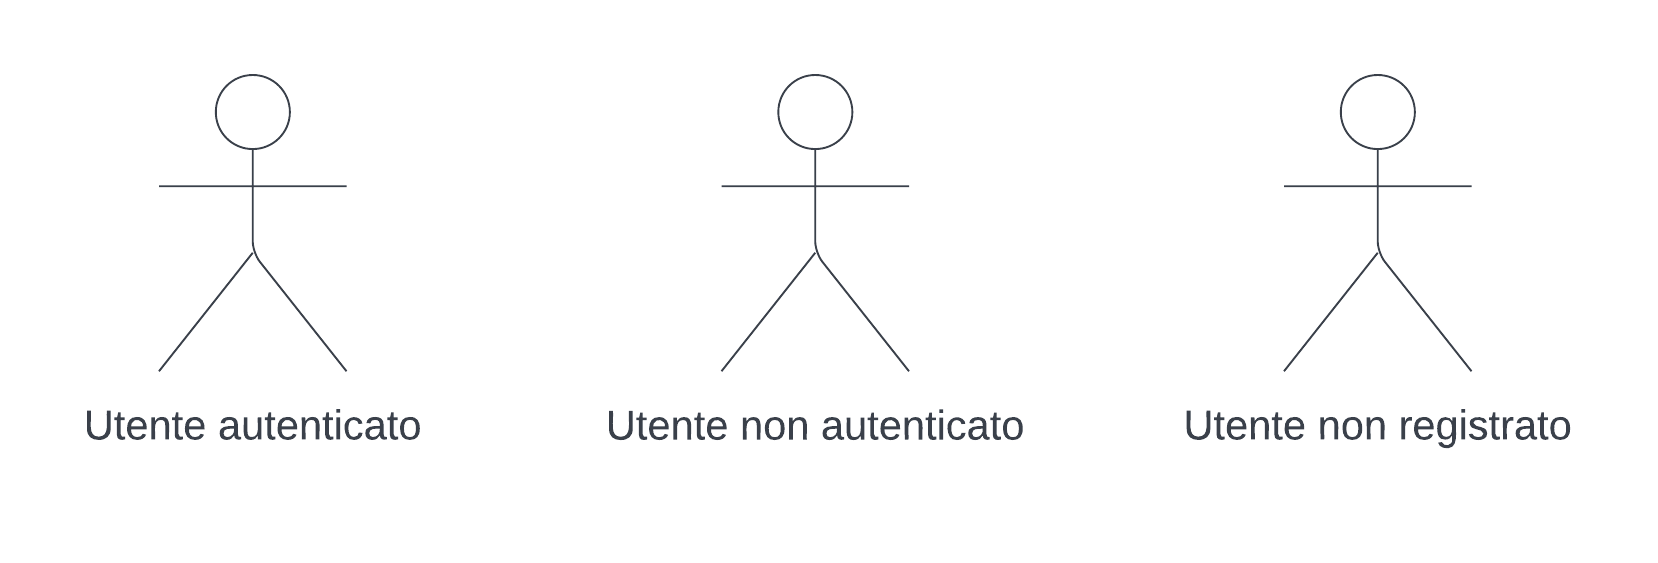
\includegraphics[width=10cm]{sezioni/Images/Actors.png}
    \centering
    \caption{Gerarchia attori}
\end{figure}
\newpage
    
\subsection{UC1 - Registrazione manuale}

\begin{figure}[!h]
    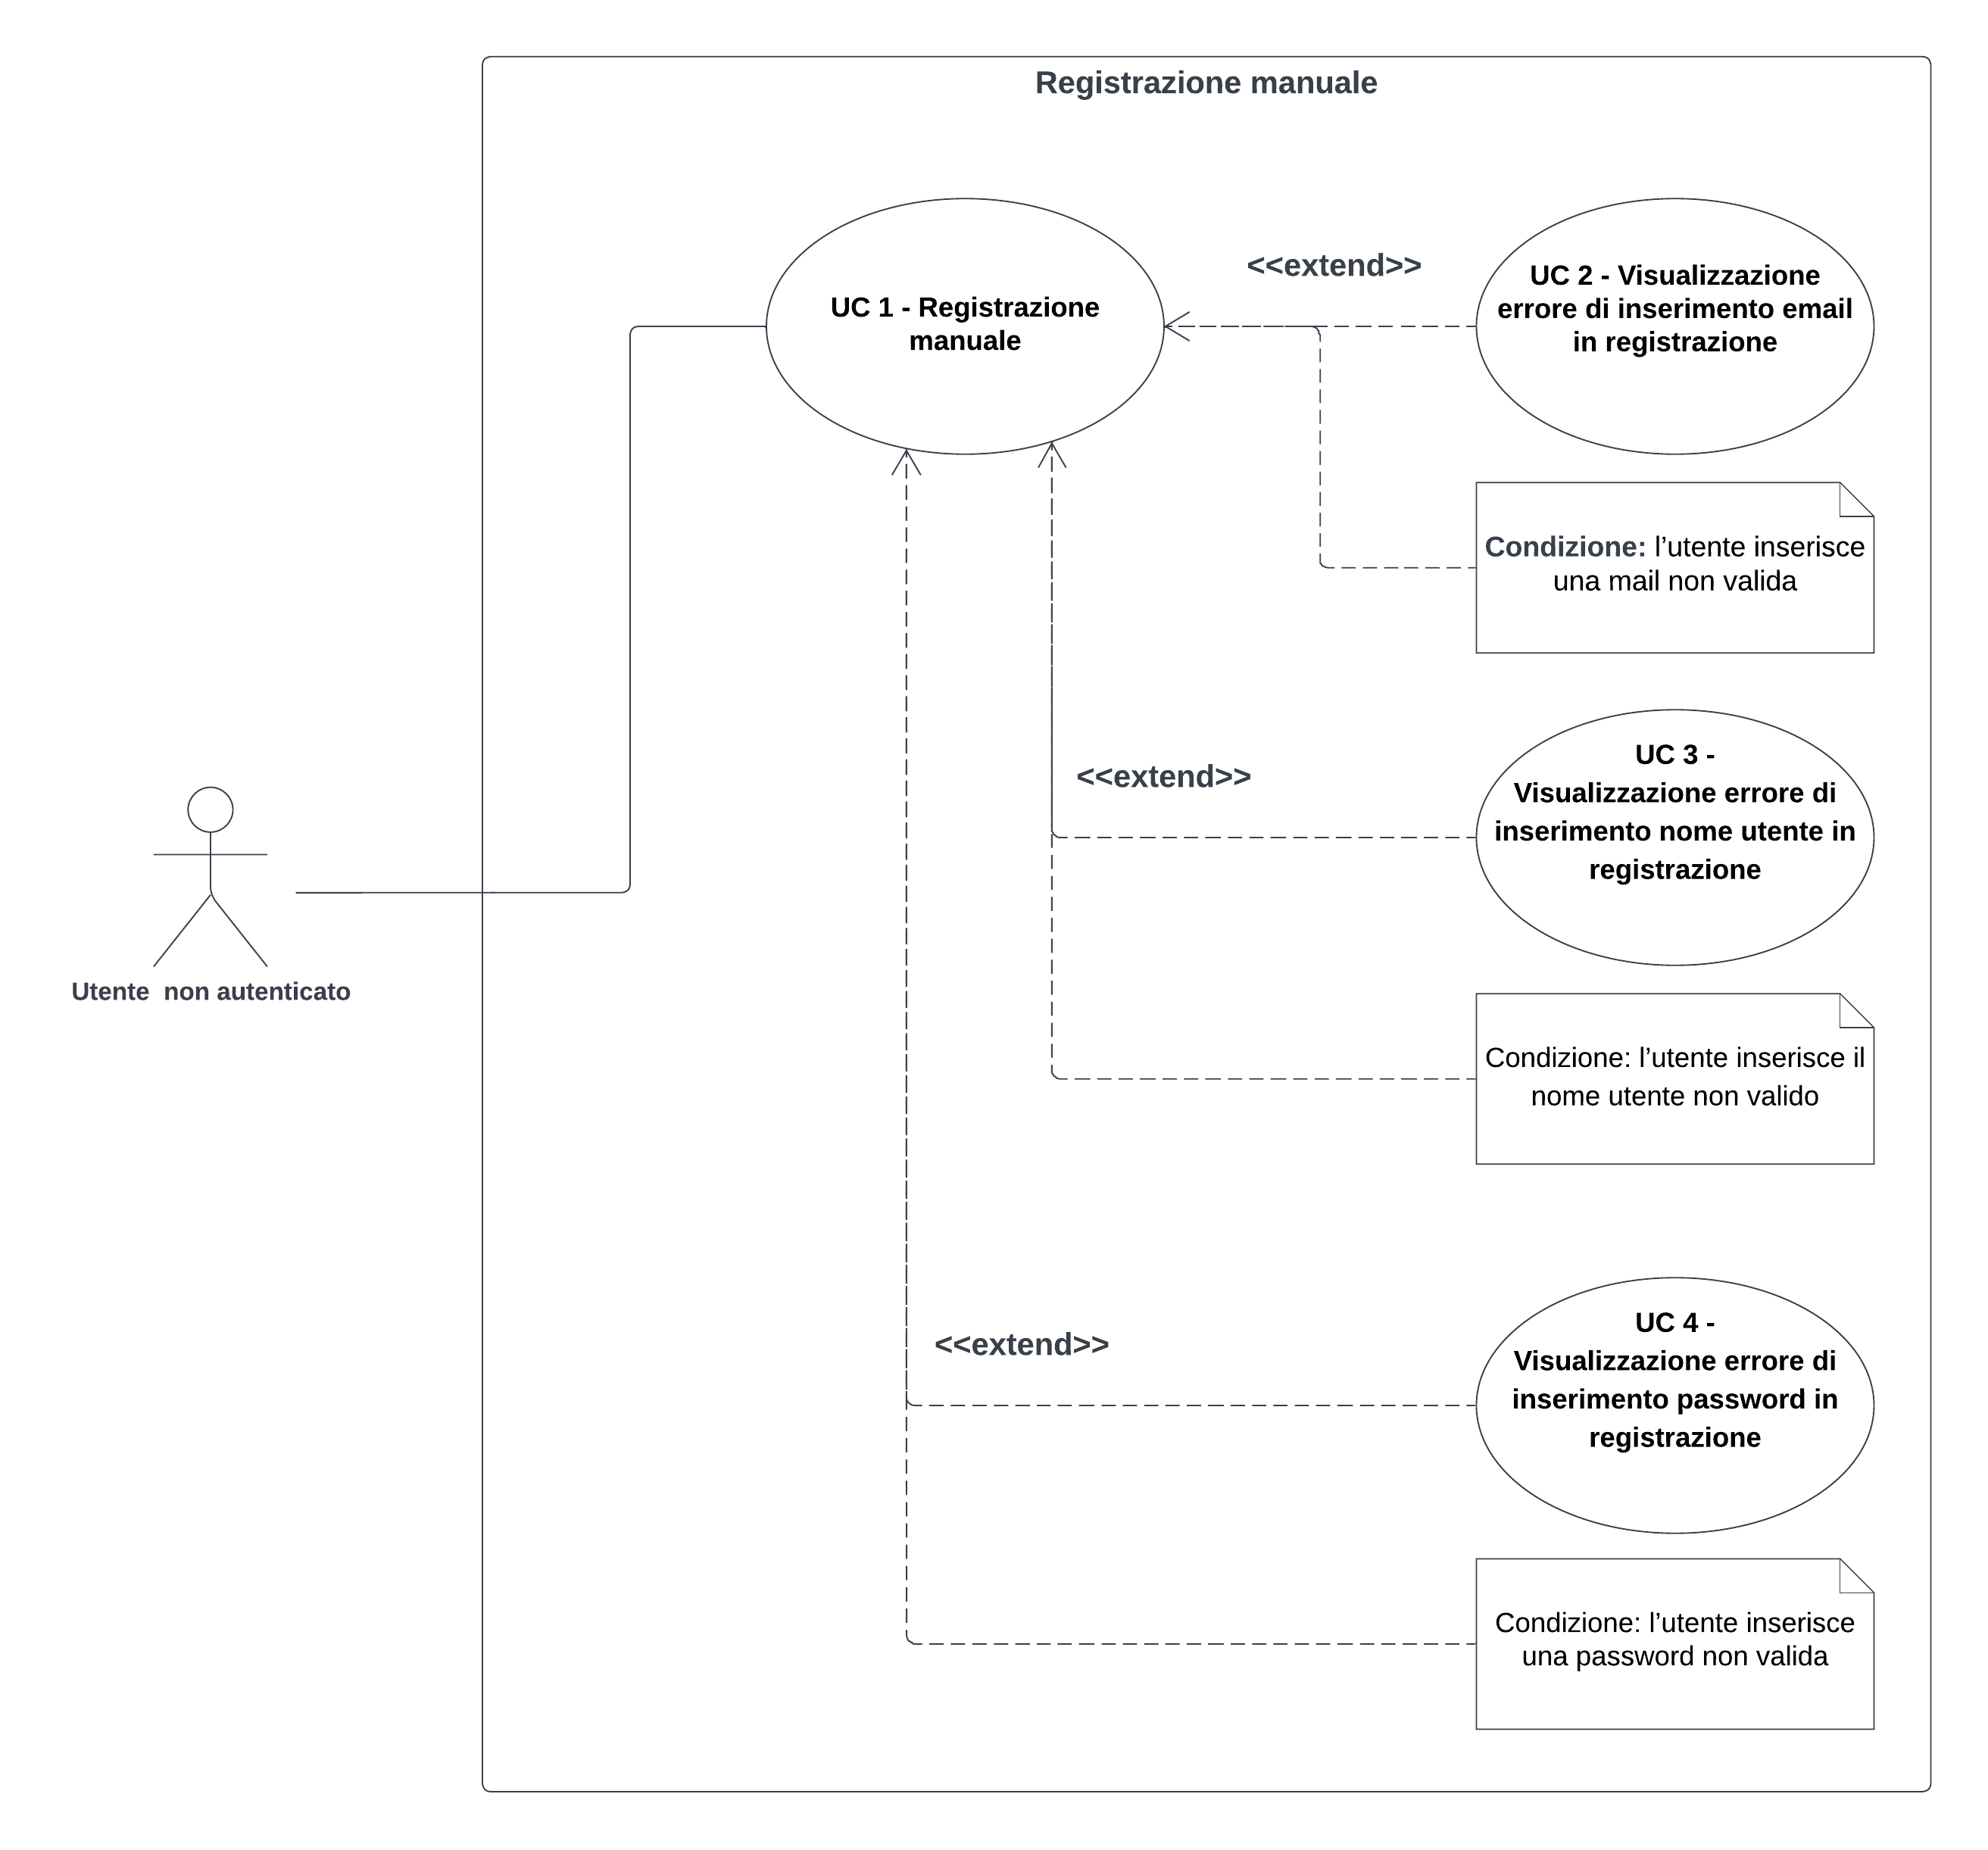
\includegraphics[width=15cm]{sezioni/Images/UC1.png}
    \centering
    \caption{UC1 - Registrazione manuale}
\end{figure}

\begin{itemize}
    \item \textbf{Attore}: utente non registrato.
    \item \textbf{Descrizione}: l'utente deve poter avere la possibilità di creare un account personale.
    \item \textbf{Scenario}:
    \begin{enumerate}
        \item l'utente si collega al sistema;
        \item l'utente clicca sul pulsante di registrazione;
        \item l'utente inserisce la propria email \textbf{(UC1.1)};
        \item l'utente inserisce il proprio nome utente \textbf{(UC1.2)};
        \item l'utente inserisce una password \textbf{(UC1.3)};
        \item l'utente conferma i dati inseriti per proseguire.
    \end{enumerate}
    \item \textbf{Estensioni}: 
        \begin{enumerate}
            \item l'utente inserisce una mail non valida  \textbf{(UC2)};
            \item l'utente inserisce il nome utente non valido \textbf{(UC3)};
            \item l'utente inserisce una password non valida \textbf{(UC4)}.
        \end{enumerate}

    \item \textbf{Precondizioni}: l'utente non è ancora registrato nel sistema.
    \item \textbf{Postcondizioni}: l'utente è registrato nel sistema.
\end{itemize}

\begin{figure}[!h]
    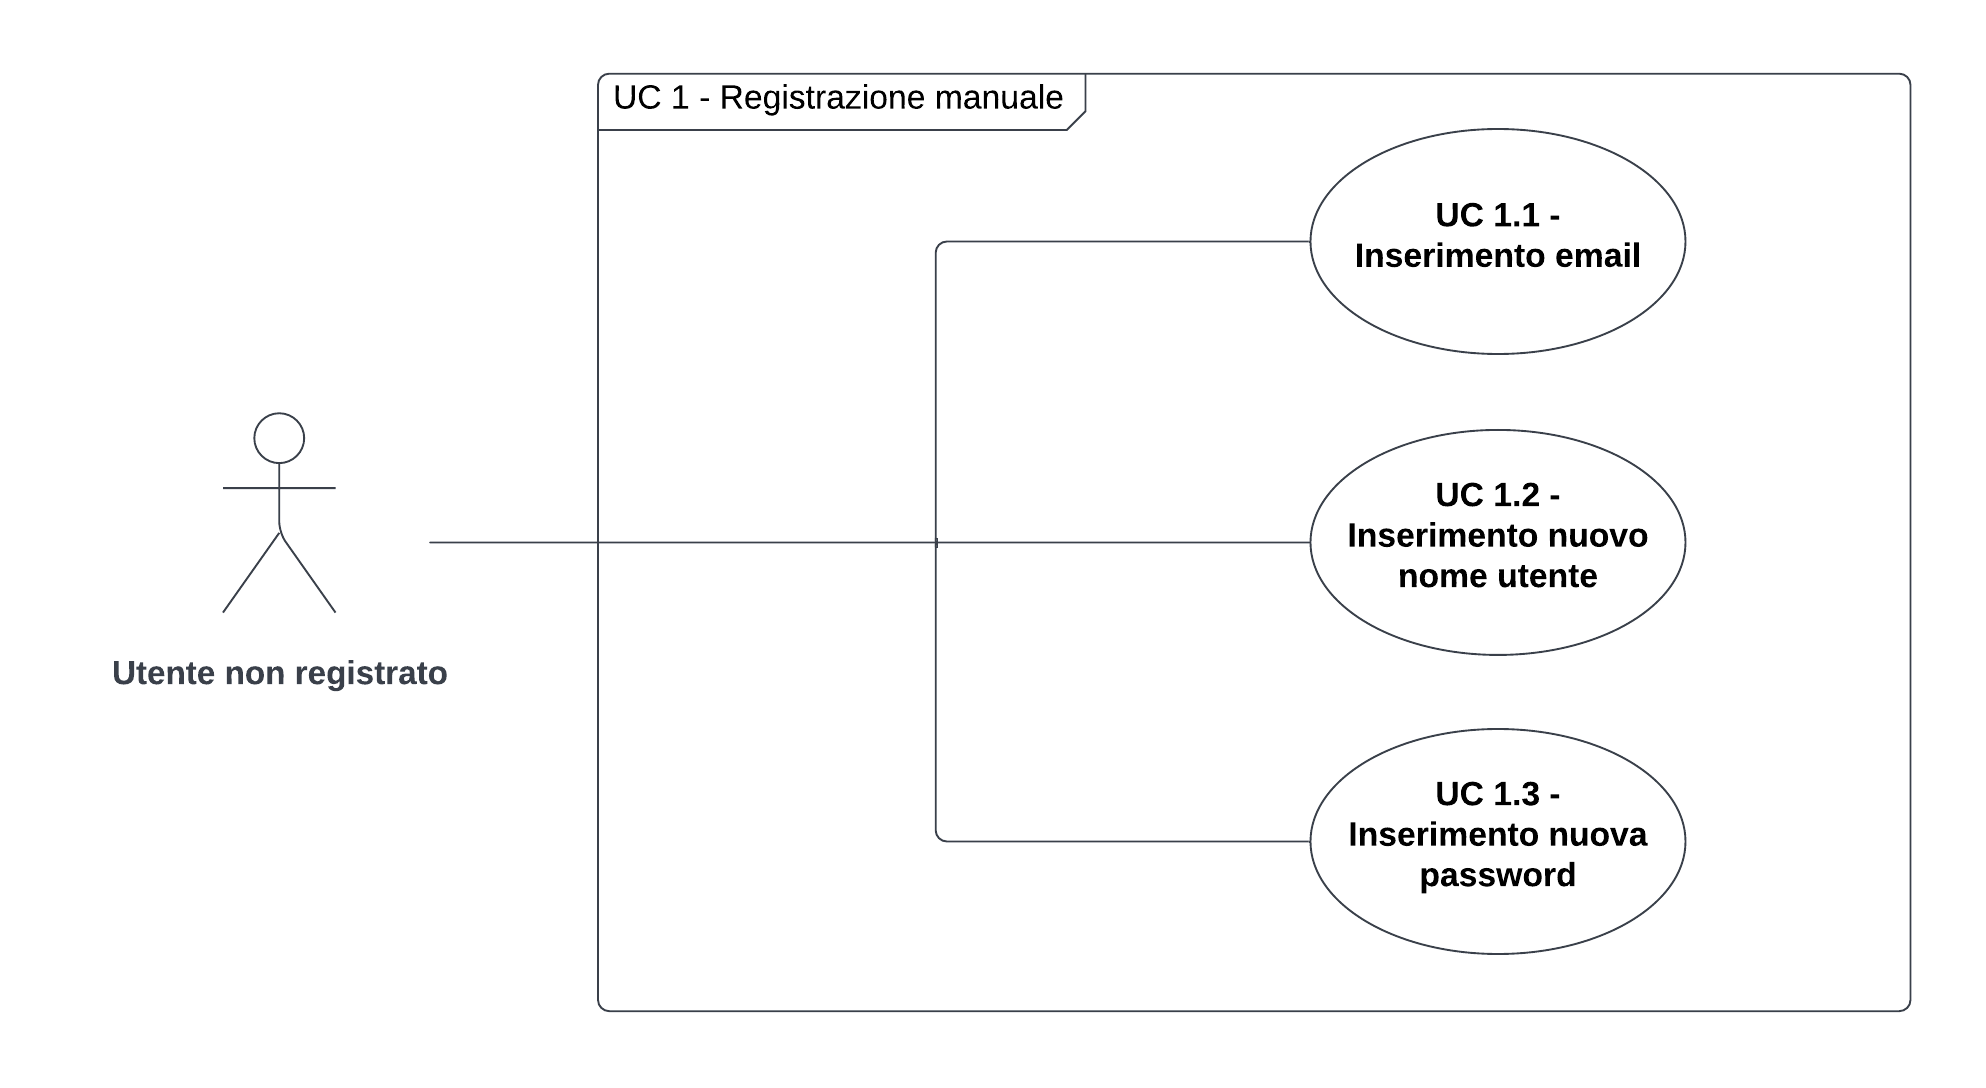
\includegraphics[width=15cm]{sezioni/Images/UC1_s.png}
    \centering
    \caption{Registrazione manuale}
\end{figure}

\subsubsection{UC1.1 - Inserimento email}
\begin{itemize}
    \item \textbf{Attore}: utente non registrato.
    \item \textbf{Descrizione}: l'utente deve avere la possibilità di inserire l'email.
    \item \textbf{Scenario}:
    \begin{enumerate}
        \item l'utente seleziona il campo relativo alla mail;
        \item l'utente inserisce la propria email.
    \end{enumerate}

    \item \textbf{Precondizioni}: l'utente effettua l'attività di registrazione.
    \item \textbf{Postcondizioni}: l'utente ha compilato il campo relativo alla mail.
\end{itemize}

\subsubsection{UC1.2 - Inserimento nuovo nome utente}
\begin{itemize}
    \item \textbf{Attore}: utente non registrato.
    \item \textbf{Descrizione}: l'utente deve avere la possibilità di creare un nuovo nome utente.
    \item \textbf{Scenario}:
    \begin{enumerate}
        \item l'utente seleziona il campo relativo il nuovo nome utente;
        \item l'utente crea il proprio nuovo nome utente.
    \end{enumerate}
    \item \textbf{Precondizioni}: l'utente effettua l'attività di registrazione.
    \item \textbf{Postcondizioni}: l'utente ha compilato il campo relativo il nuovo nome utente.
\end{itemize}

\subsubsection{UC1.3 - Inserimento nuova password}
\begin{itemize}
    \item \textbf{Attore}: utente non registrato.
    \item \textbf{Descrizione}: l'utente deve avere la possibilità di creare una nuova password.
    \item \textbf{Scenario}:
    \begin{enumerate}
        \item l'utente seleziona il campo relativo la nuova password;
        \item l'utente crea la nuova password.
    \end{enumerate}

    \item \textbf{Precondizioni}: l'utente effettua l'attività di registrazione.
    \item \textbf{Postcondizioni}: l'utente ha compilato il campo relativo la nuova password.
\end{itemize}

\subsection{UC2 - Visualizzazione errore di inserimento email in registrazione}
\begin{itemize}
    \item \textbf{Attore}: utente non registrato.
    \item \textbf{Descrizione}: l'utente deve essere notificato con un errore nel caso in cui le informazioni inserite nel campo email siano invalide.
    \item \textbf{Scenario}: l'utente visualizza un messaggio di errore.
    \item \textbf{Precondizioni}: l'utente inserisce una mail non valida nell'apposito input box.
    \item \textbf{Postcondizioni}: l'utente riceve il messaggio di errore.
\end{itemize}

\subsection{UC3 - Visualizzazione errore di inserimento nome utente in registrazione}
\begin{itemize}
    \item \textbf{Attore}: utente non registrato.
    \item \textbf{Descrizione}: l'utente deve essere notificato con un errore nel caso in cui venga inserito un nome utente non valido.
    \item \textbf{Scenario}: l'utente visualizza un messaggio di errore.
    \item \textbf{Precondizioni}: l'utente inserisce un nome utente non valido nell'apposito input box.
    \item \textbf{Postcondizioni}: l'utente riceve il messaggio di errore.
\end{itemize}

\subsection{UC4 - Visualizzazione errore di inserimento password in registrazione}
\begin{itemize}
    \item \textbf{Attore}: utente non registrato.
    \item \textbf{Descrizione}: l'utente deve essere notificato con un errore nel caso in cui inserisca una password non valida durante la fase di registrazione.
    \item \textbf{Scenario}: l'utente visualizza un messaggio di errore.
    \item \textbf{Precondizioni}: l'utente inserisce una password non valida nell'apposito input box.
    \item \textbf{Postcondizioni}: l'utente riceve il messaggio di errore.
\end{itemize}

\subsection{UC5 - Login}
\begin{figure}[!h]
    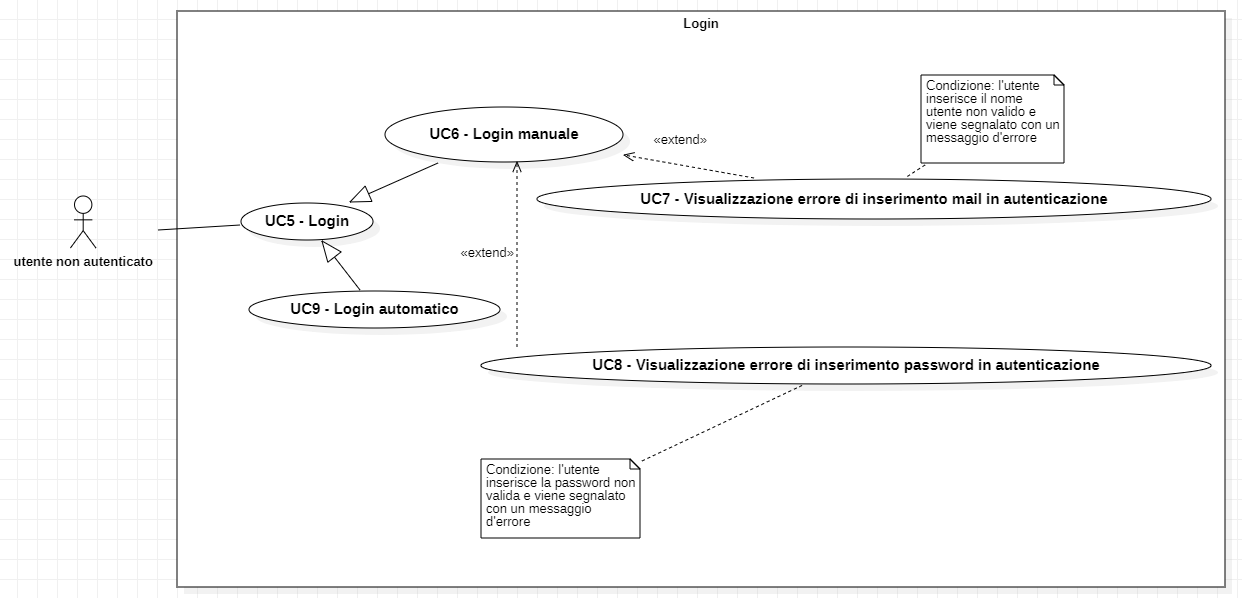
\includegraphics[width=15cm]{sezioni/Images/UC5-log.png}
    \centering
    \caption{UC5 - Login}
\end{figure}
\begin{itemize}
    \item \textbf{Attore}: l'utente non è autenticato.
    \item \textbf{Descrizione}: l'utente deve poter autenticarsi e accedere al proprio account.
    \item \textbf{Scenario}:
    \begin{enumerate}
        \item l'utente si collega al sistema;
        \item l'utente clicca sul pulsante di login;
        \item l'utente si collega manualmente \textbf{(UC6)} oppure automaticamente \textbf{(UC9)}.
    \end{enumerate}
    \item \textbf{Precondizioni}: l'utente non è ancora autenticato al sistema.
    \item \textbf{Postcondizioni}: l'utente si è autenticato al sistema.
\end{itemize}

\subsection{UC6 - Login manuale}

\begin{itemize}
    \item \textbf{Attore}: l'utente non è autenticato.
    \item \textbf{Descrizione}: l'utente accedendo con l'account personale, deve poter autenticarsi.
    \item \textbf{Scenario}:
    \begin{enumerate}
        \item l'utente si collega al sistema;
        \item l'utente clicca sul pulsante di login;
        \item l'utente inserisce il proprio nome utente \textbf{(UC6.1)};
        \item l'utente inserisce la propria password \textbf{(UC6.2)};
        \item l'utente decide se memorizzare la sessione \textbf{(UC6.3 )};
        \item l'utente clicca il pulsante di conferma per proseguire.
    \end{enumerate}
    \item \textbf{Estensioni}:
        \begin{enumerate}
            \item l'utente inserisce il nome utente non valido e viene segnalato con un messaggio d'errore \textbf{(UC 7)};
            \item l'utente inserisce la password non valida e viene segnalato con un messaggio d'errore \textbf{(UC 8)};
        \end{enumerate}

    \item \textbf{Precondizioni}: l'utente non è ancora autenticato.
    \item \textbf{Postcondizioni}: l'utente si è autenticato al sistema.
\end{itemize}

\begin{figure}[!h]
    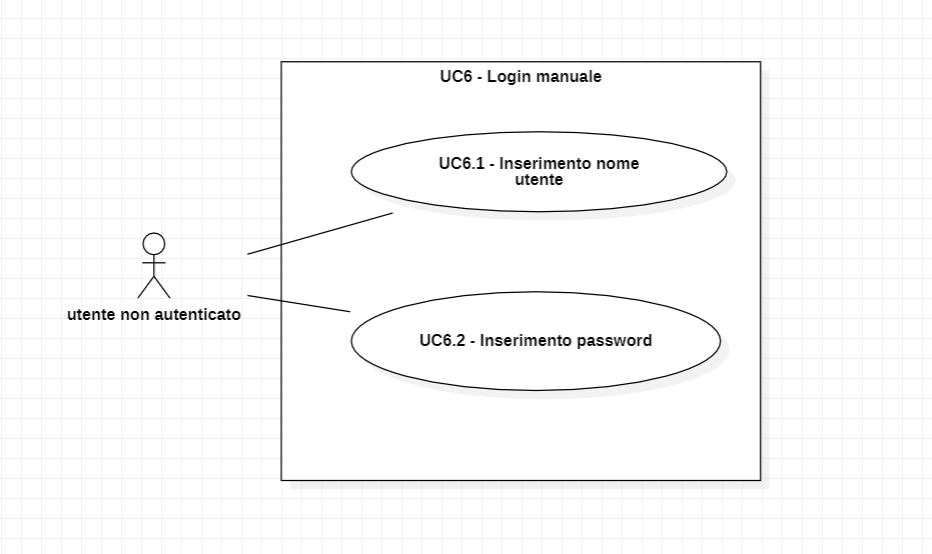
\includegraphics[width=10cm]{sezioni/Images/UC6-Manuale.png}
    \centering
    \caption{UC6 - Login manuale}
\end{figure}

\subsubsection{UC6.1 - Inserimento nome utente}
\begin{itemize}
    \item \textbf{Attore}: utente non autenticato.
    \item \textbf{Descrizione}: l'utente deve poter inserire il nome utente per autenticarsi.
    \item \textbf{Scenario}:
    \begin{enumerate}
        \item l'utente seleziona il campo relativo al nome utente;
        \item l'utente inserisce il nome utente.
    \end{enumerate}
    \item \textbf{Precondizioni}: l'utente effettua l'attività di autenticazione.
    \item \textbf{Postcondizioni}: l'utente ha compilato il campo relativo il nome utente.
\end{itemize}

\subsubsection{UC6.2 - Inserimento password}
\begin{itemize}
    \item \textbf{Attore}: utente non autenticato.
    \item \textbf{Descrizione}: l'utente deve poter inserire la password per autenticarsi.
    \item \textbf{Scenario}:
    \begin{enumerate}
        \item l'utente seleziona il campo relativo alla password;
        \item l'utente inserisce la password.
    \end{enumerate}

    \item \textbf{Precondizioni}: l'utente effettua l'attività di autenticazione.
    \item \textbf{Postcondizioni}: l'utente ha compilato il campo relativo il nome utente.
\end{itemize}

\subsubsection{UC6.3 Memorizzazione sessione}
\begin{itemize}
    \item \textbf{Attore}: utente non autenticato.
    \item \textbf{Descrizione}: l'utente deve poter memorizzare la sessione.
    \item \textbf{Scenario}: l'utente spunta la casella per mantenere memorizzata la sessione.
    \item \textbf{Precondizioni}: l'utente effettua l'attività di autenticazione.
    \item \textbf{Postcondizioni}: l'utente ha chiesto che la sessione venga memorizzata.
\end{itemize}

\subsection{UC7 - Visualizzazione errore di inserimento mail in autenticazione}
\begin{itemize}
    \item \textbf{Attore}: utente non autenticato.
    \item \textbf{Descrizione}: l'utente deve essere notificato con un errore nel caso in cui l'email inserita sia invalida durante la fase di autenticazione.
    \item \textbf{Scenario}: l'utente visualizza un messaggio di errore. 
    \item \textbf{Precondizioni}: l'utente effettua l'attività di autenticazione ed inserisce l'email non valida.
    \item \textbf{Postcondizioni}: l'utente riceve il messaggio di errore.
\end{itemize}

\subsection{UC8 - Visualizzazione errore di inserimento password in autenticazione} 
\begin{itemize}
    \item \textbf{Attore}: utente non autenticato.
    \item \textbf{Descrizione}: l'utente deve essere notificato con un errore nel caso in cui la password inserita sia invalida durante la fase di autenticazione.
    \item \textbf{Scenario}: l'utente visualizza un messaggio di errore. 
    \item \textbf{Precondizioni}: l'utente effettua l'attività di autenticazione ed inserisce la password non valida.
    \item \textbf{Postcondizioni}: l'utente riceve il messaggio di errore.
\end{itemize}

\subsection{UC9 - Login automatico}
\begin{itemize}
    \item \textbf{Attore}: utente non autenticato.
    \item \textbf{Descrizione}: l'utente accedendo con l'account personale, deve poter autenticarsi automaticamente se la sessione rimane memorizzata.
    \item \textbf{Scenario}:
    \begin{enumerate}
        \item l'utente si collega al sistema;
        \item l'utente viene automaticamente autenticato.
    \end{enumerate}

    \item \textbf{Precondizioni}: l'utente ha una sessione attiva memorizzata.
    \item \textbf{Postcondizioni}: l'utente si è autenticato al sistema.
\end{itemize}

\subsection{UC10 - Logout}
\begin{itemize}
    \item \textbf{Attore}: l'utente è autenticato.
    \item \textbf{Descrizione}: l'utente deve poter uscire dalla sessione.
    \item \textbf{Scenario}:
    \begin{enumerate}
        \item l'utente è collegato al sistema;
        \item l'utente clicca il pulsante di logout.
    \end{enumerate}

    \item \textbf{Precondizioni}: l'utente è autenticato.
    \item \textbf{Postcondizioni}: l'utente non è più autenticato al sistema.
\end{itemize}

\subsection{UC11 - Modifica password}

\begin{figure}[H]
    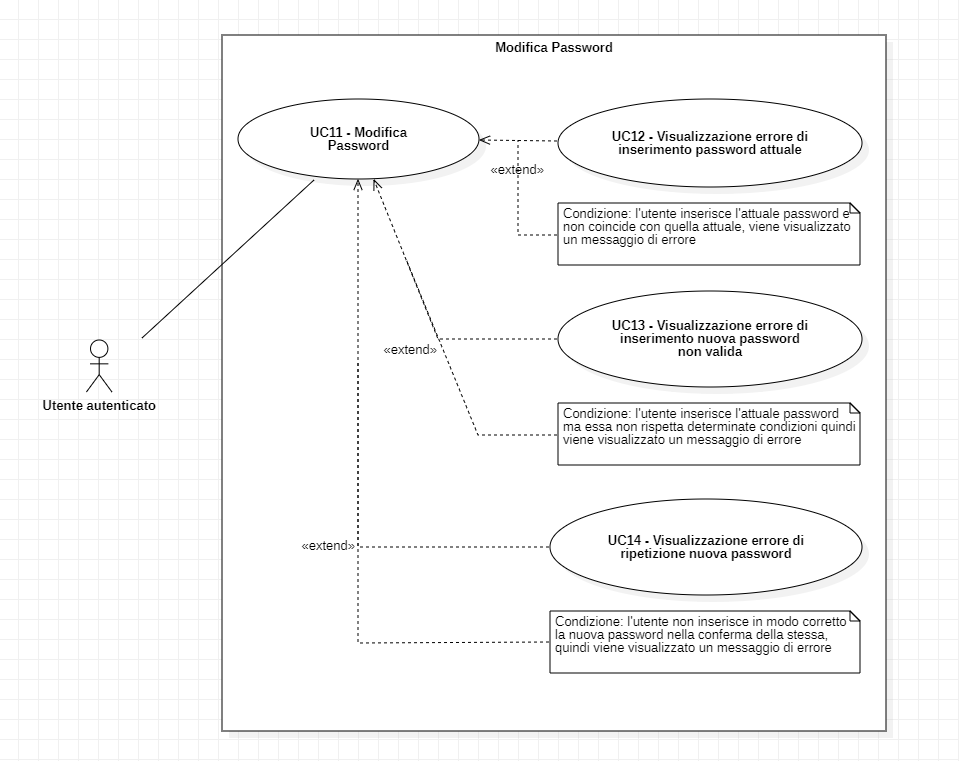
\includegraphics[width=15cm]{sezioni/Images/UC11.png}
    \centering
    \caption{Modifica password}
\end{figure}

\begin{itemize}
    \item \textbf{Attore}: l'utente è autenticato.
    \item \textbf{Descrizione}: l'utente deve poter modificare l'attuale password, con la quale effettua il login.
    \item \textbf{Scenario}:
    \begin{enumerate}
        \item inserimento password attuale;
        \item inserimento nuova password;
        \item conferma nuova password;
        \item conferma modifica password.
    \end{enumerate}
    \textbf{Estensioni}:
    \begin{enumerate}
        \item l'utente inserisce l'attuale password e non coincide con quella attuale, viene visualizzato un messaggio di errore \textbf{(UC12)};
        \item l'utente inserisce la nuova password ma essa non rispetta determinate condizioni quindi viene visualizzato un messaggio di errore \textbf{(UC13)};
        \item l'utente non inserisce in modo corretto la nuova password nella conferma della stessa, quindi viene visualizzato un messaggio di errore \textbf{(UC14)};
    \end{enumerate}

    \item \textbf{Precondizioni}: l'utente è autenticato con una determinata password.
    \item \textbf{Postcondizioni}: l'utente è autenticato con una nuova password.
\end{itemize}

\begin{figure}[!h]
    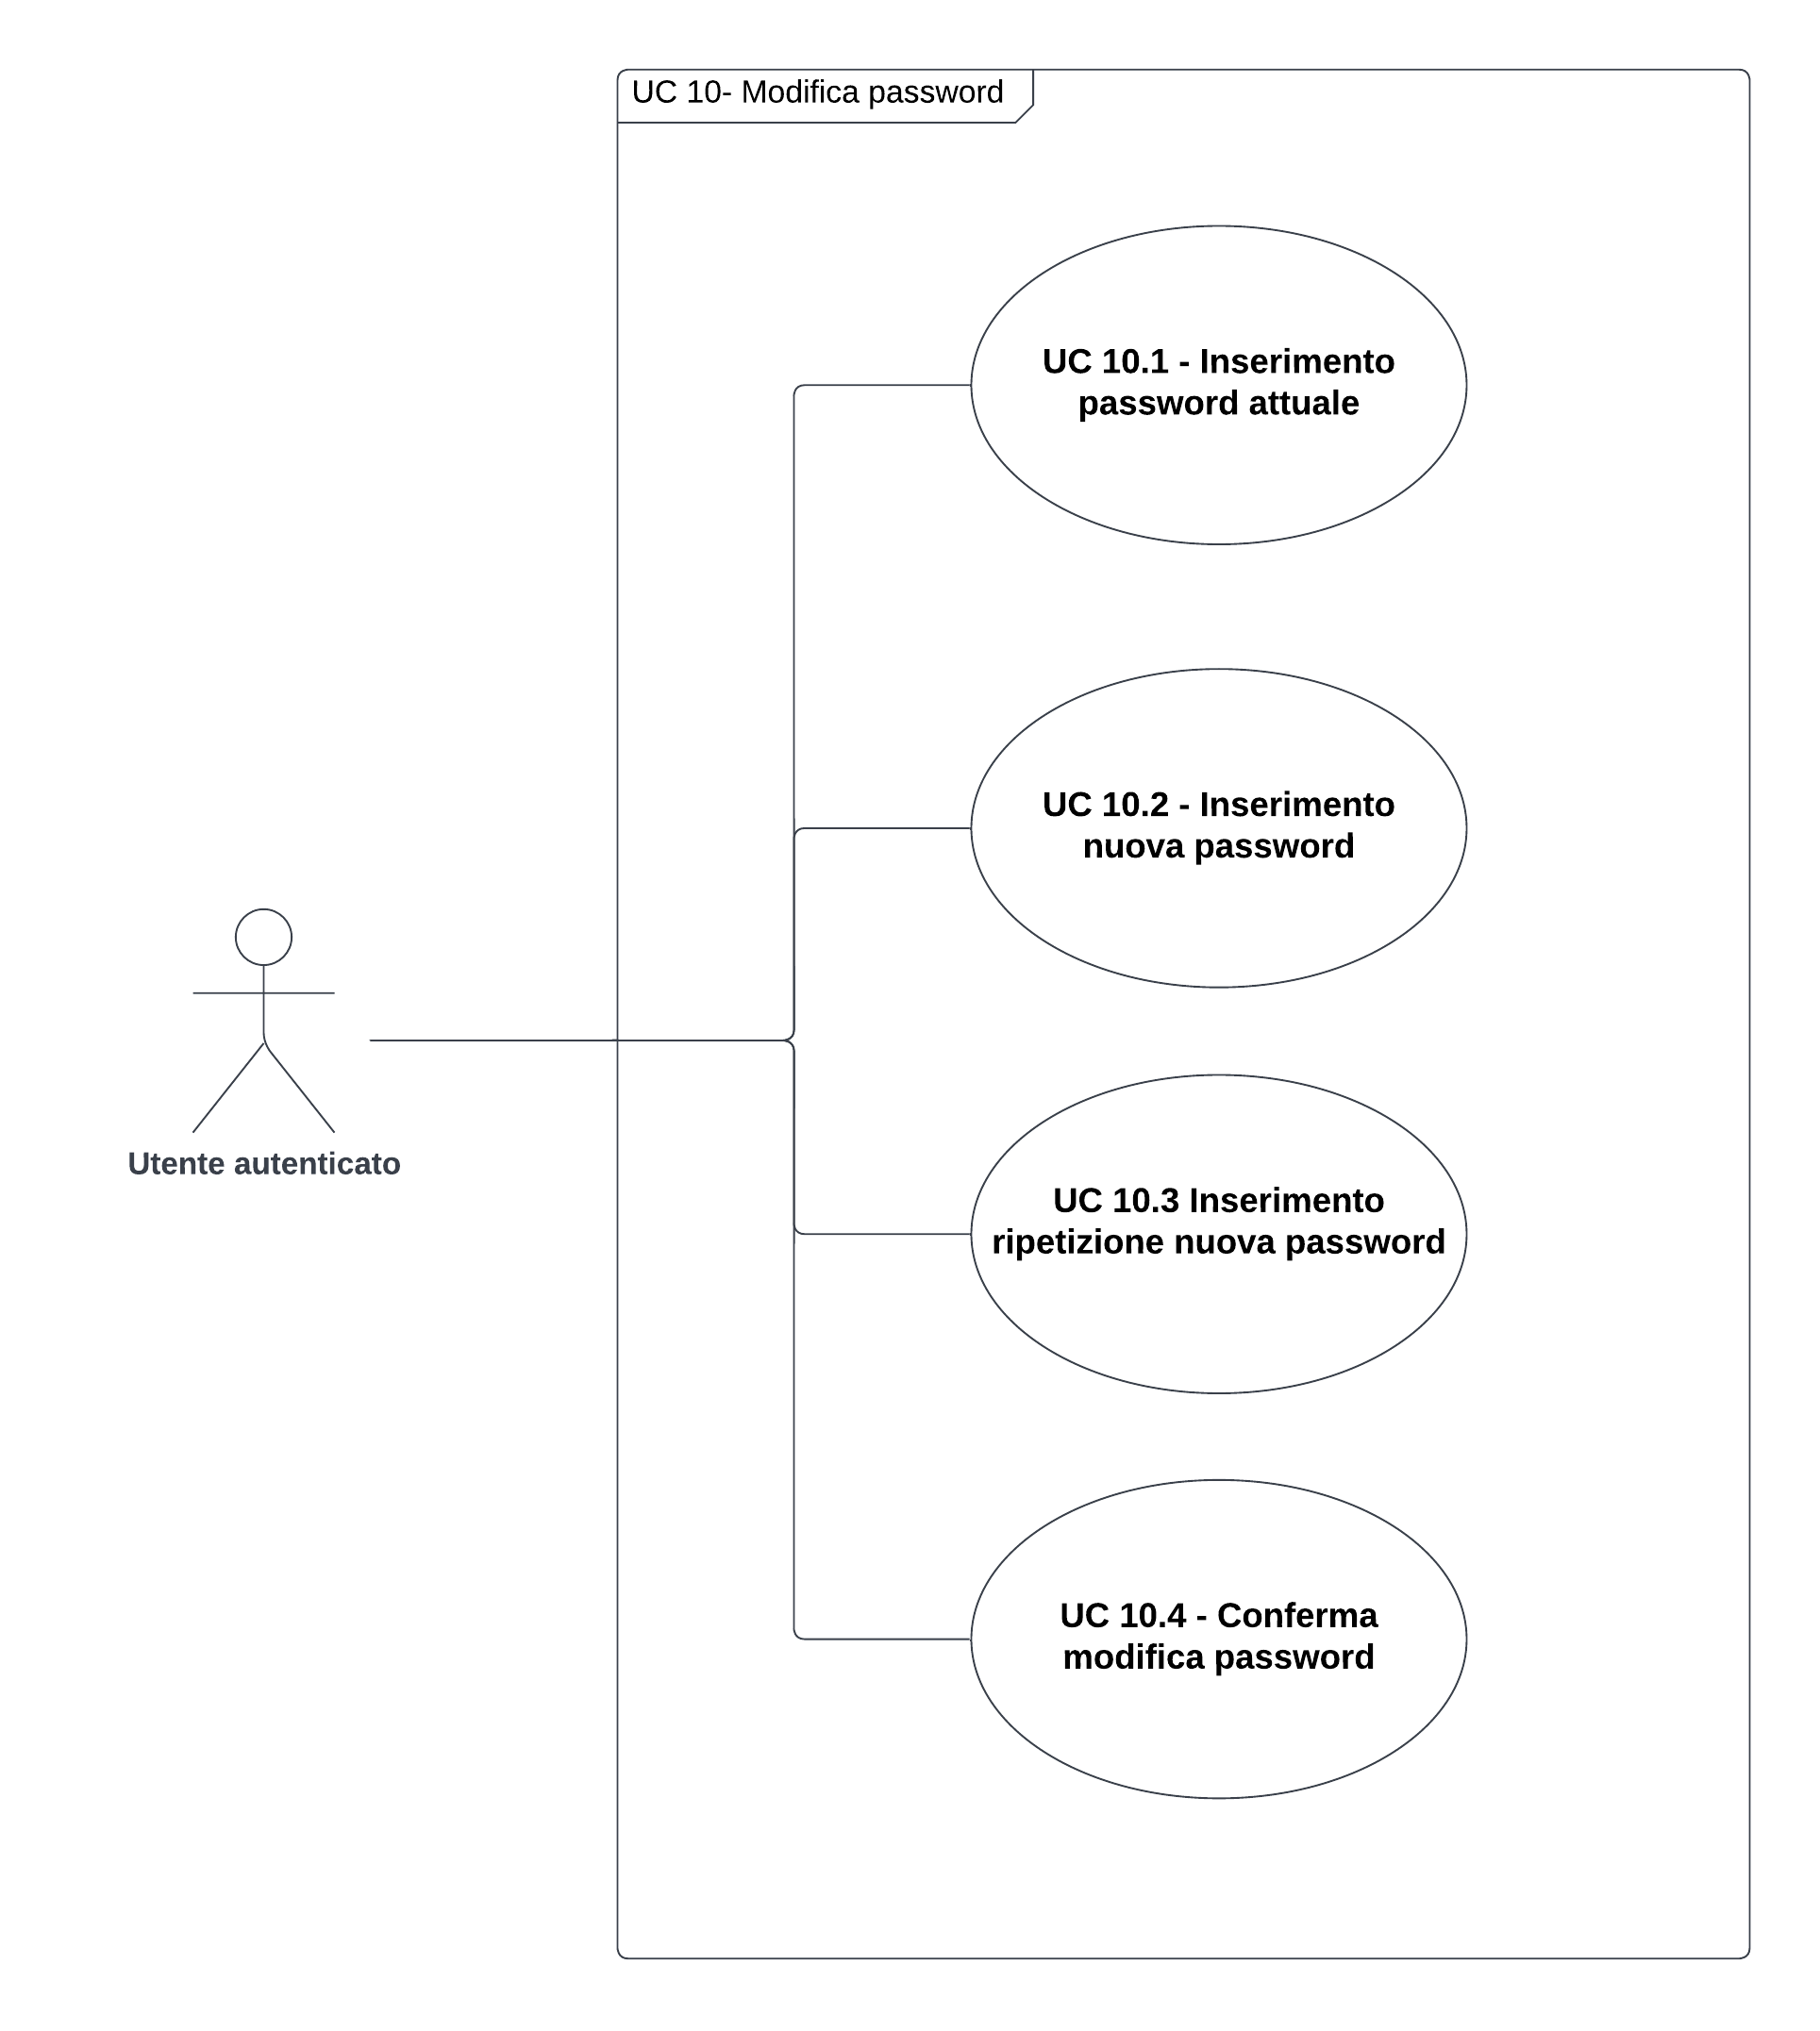
\includegraphics[width=15cm]{sezioni/Images/UC10_s.png}
    \centering
    \caption{Modifica password}
\end{figure}

\subsubsection{UC11.1 - Inserimento password attuale} 
\begin{itemize}
    \item \textbf{Attore}: l'utente è autenticato.
    \item \textbf{Descrizione}: l'utente deve inserire la password attuale durante la sessione di “modifica password”.
    \item \textbf{Scenario}:
    \begin{enumerate}
        \item l'utente seleziona il campo riferito alla password attuale;
        \item l'utente inserisce la password attuale.
    \end{enumerate}

    \item \textbf{Precondizioni}: l'utente svolge la sessione di modifica password.
    \item \textbf{Postcondizioni}: l'utente ha inserito la propria password attuale.

\end{itemize}

\subsubsection{UC11.2 - Inserimento nuova password}
\begin{itemize}
    \item \textbf{Attore}: l'utente è autenticato.
    \item \textbf{Descrizione}: durante l'attività di modifica della password l'utente deve poter inserire la nuova password.
    \item \textbf{Scenario}:
    \begin{enumerate}
        \item l'utente seleziona il campo riferito alla nuova password;
        \item l'utente inserisce la nuova password.
    \end{enumerate}

    \item \textbf{Precondizioni}: l'utente svolge la sessione di modifica password.
    \item \textbf{Postcondizioni}: l'utente ha inserito la nuova password.
\end{itemize}

\subsubsection{UC11.3 - Inserimento ripetizione nuova password}
\begin{itemize}
    \item \textbf{Attore}: l'utente è autenticato.
    \item \textbf{Descrizione}: durante l'attività di modifica password l'utente deve poter inserire la ripetizione della nuova password.
    \item \textbf{Scenario}:
    \begin{enumerate}
        \item l'utente seleziona il campo riferito alla ripetizione della nuova password;
        \item l'utente inserisce la ripetizione della nuova password.
    \end{enumerate}

    \item \textbf{Precondizioni}: l'utente svolge la sessione di modifica password.
    \item \textbf{Postcondizioni}: l'utente ha inserito la ripetizione della nuova password.
\end{itemize}

\subsubsection{UC11.4 - Conferma modifica password}
\begin{itemize}
    \item \textbf{Attore}: l'utente è autenticato.
    \item \textbf{Descrizione}: durante l'attività di modifica password l'utente deve poter confermare la nuova password.
    \item \textbf{Scenario}: l'utente conferma la nuova password inserita. 
    \item \textbf{Precondizioni}: l'utente svolge la sessione di modifica password.
    \item \textbf{Postcondizioni}: l'utente ha provato a modificare la propria password.
\end{itemize}

\subsection{UC12 - Visualizzazione errore di inserimento password attuale}
\begin{itemize}
    \item \textbf{Attore}: l'utente è autenticato.
    \item \textbf{Descrizione}: durante l'attività di modifica password l'utente deve ricevere un messaggio d'errore se l'inserimento della password attuale non è andato a buon fine.
    \item \textbf{Scenario}: l'utente legge un messaggio d'errore. 
    \item \textbf{Precondizioni}: l'utente svolge la sessione di modifica password e la password attuale inserita non è corretta.
    \item \textbf{Postcondizioni}: l'utente ha ricevuto un messaggio d'errore.
\end{itemize}

\subsection{UC13 - Visualizzazione errore di inserimento nuova password non valida}
\begin{itemize}
    \item \textbf{Attore}: l'utente è autenticato.
    \item \textbf{Descrizione}: durante l'attività di modifica password l'utente deve ricevere un messaggio d'errore se l'inserimento di una nuova password non è valida.
    \item \textbf{Scenario}: l'utente legge un messaggio d'errore. 
    \item \textbf{Precondizioni}: l'utente svolge la sessione di modifica password e la nuova password inserita non è valida.
    \item \textbf{Postcondizioni}: l'utente ha ricevuto un messaggio d'errore.

\end{itemize}

\subsection{UC14 - Visualizzazione errore di ripetizione nuova password}
\begin{itemize}
    \item \textbf{Attore}: l'utente è autenticato.
    \item \textbf{Descrizione}: durante l'attività di modifica password l'utente deve ricevere un messaggio d'errore se l'inserimento della ripetizione della nuova password non è uguale alla nuova password.
    \item \textbf{Scenario}: l'utente legge un messaggio d'errore. 
    \item \textbf{Precondizioni}: l'utente svolge la sessione di modifica password e la ripetizione della nuova password inserita non è corretta.
    \item \textbf{Postcondizioni}: l'utente ha ricevuto un messaggio d'errore.
\end{itemize}

\subsection{UC15 - Visualizzazione guida}

\begin{figure}[H]
    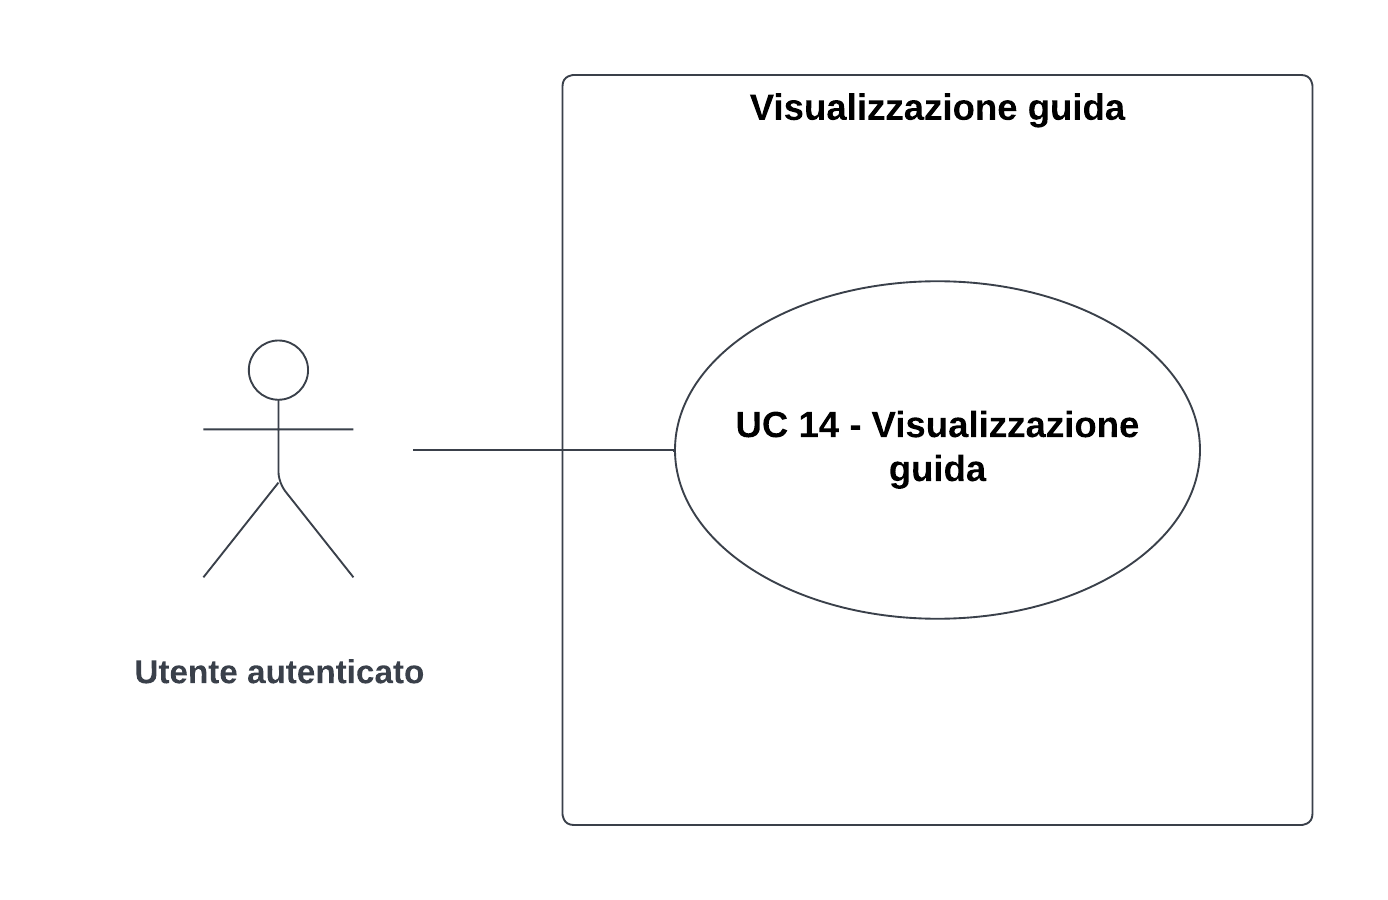
\includegraphics[width=10cm]{sezioni/Images/UC14.png}
    \centering
    \caption{Visualizzazione guida}
\end{figure}

\begin{itemize}
    \item \textbf{Attore}: l'utente è autenticato.
    \item \textbf{Descrizione}: l'utente deve poter visualizzare la guida in formato mappa o formato lista.
    \item \textbf{Scenario}: l'utente si trova nella home.
    \item \textbf{Precondizioni}: l'utente vuole visualizzare la guida.
    \item \textbf{Postcondizioni}: l'utente visualizza la guida.
\end{itemize}

\begin{figure}[H]
    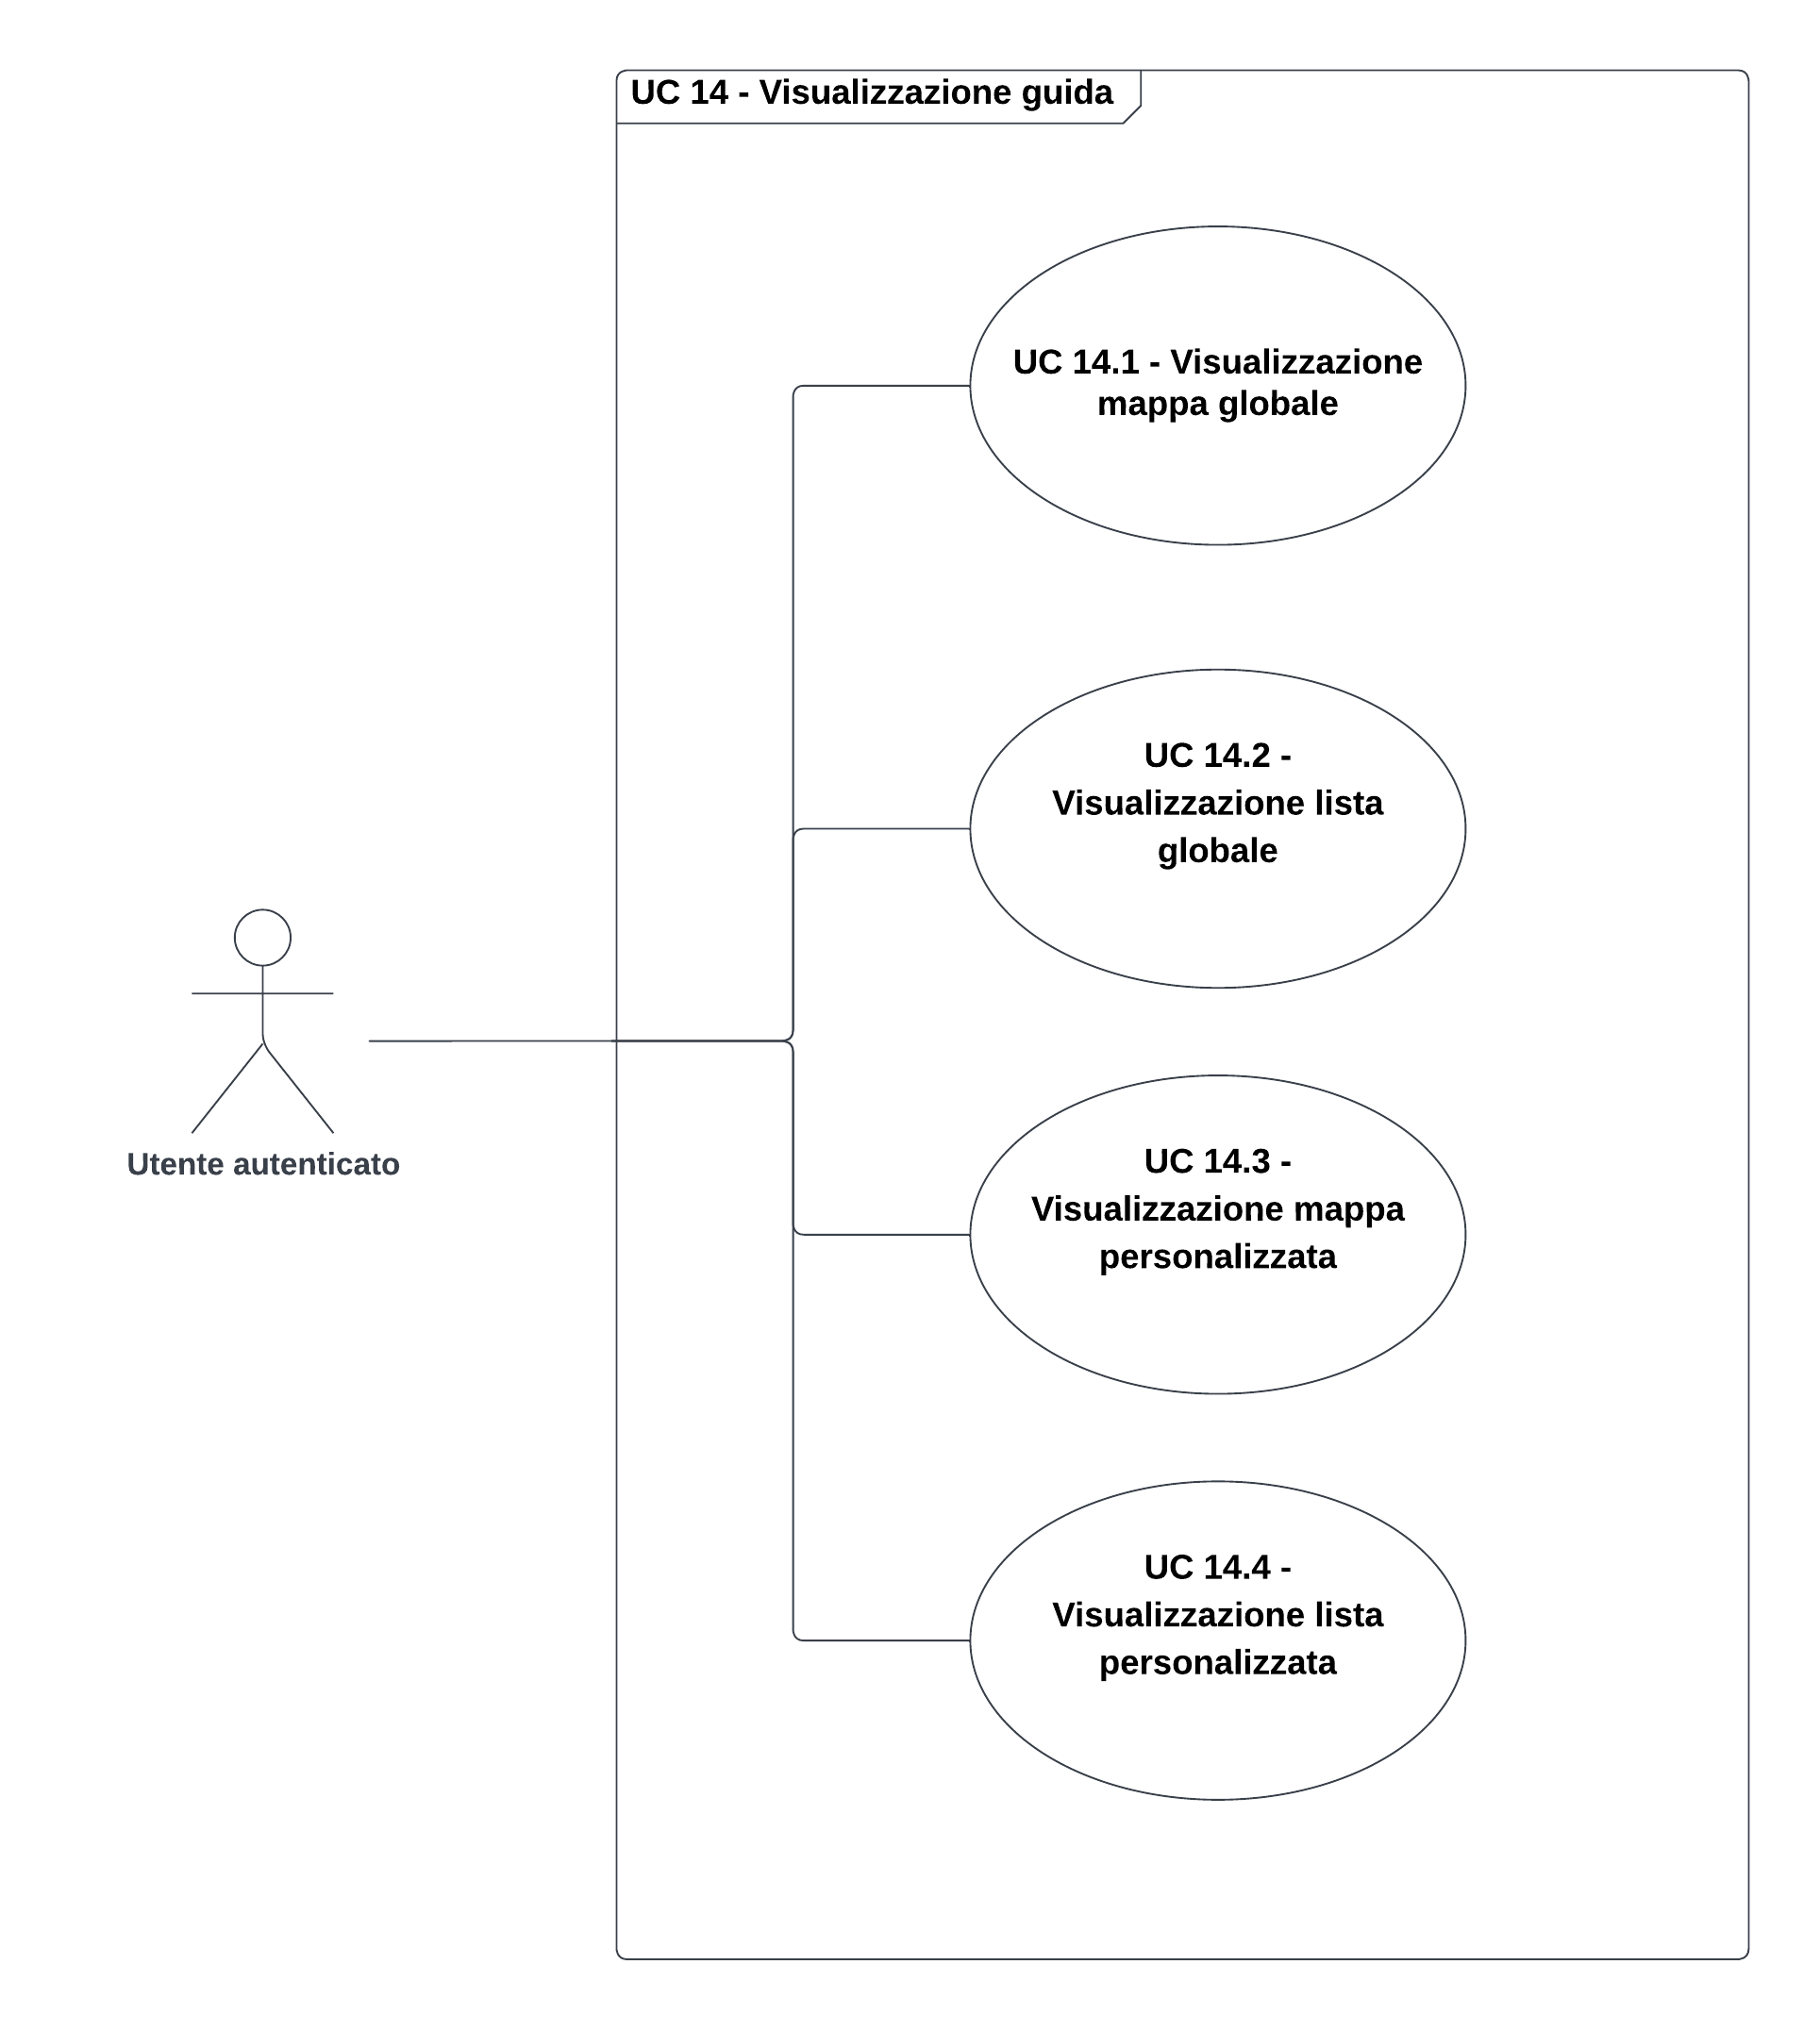
\includegraphics[width=13cm]{sezioni/Images/UC14_s.png}
    \centering
    \caption{Visualizzazione guida}
\end{figure}

\subsubsection{UC15.1 - Visualizzazione mappa globale}
\begin{itemize}
    \item \textbf{Attore}: l'utente è autenticato.
    \item \textbf{Descrizione}: l'utente visualizza la mappa globale se non ha nessun profilo social seguito.
    \item \textbf{Scenario}:
    \begin{enumerate}
        \item l'utente non segue nessun profilo social;
        \item l'utente visualizza la mappa globale nella home.
    \end{enumerate}

    \item \textbf{Precondizioni}: l'utente vuole visualizzare la mappa globale.
    \item \textbf{Postcondizioni}: l'utente visualizza la mappa globale.
\end{itemize}

\subsubsection{UC15.2 - Visualizzazione lista globale}
\begin{itemize}
    \item \textbf{Attore}: l'utente è autenticato.
    \item \textbf{Descrizione}: l'utente visualizza la lista globale se non ha nessun profilo social seguito.
    \item \textbf{Scenario}:
    \begin{enumerate}
        \item l'utente non segue nessun profilo social;
        \item l'utente visualizza la lista globale nella home.
    \end{enumerate}

    \item \textbf{Precondizioni}: l'utente vuole visualizzare la lista globale.
    \item \textbf{Postcondizioni}: l'utente visualizza la lista globale.
\end{itemize}

\subsubsection{UC15.3 - Visualizzazione mappa personalizzata}
\begin{itemize}
    \item \textbf{Attore}: l'utente è autenticato.
    \item \textbf{Descrizione}: l'utente visualizza la mappa personalizzata se ha dei profili social seguiti.
    \item \textbf{Scenario}:
    \begin{enumerate}
        \item l'utente segue dei profilo social;
        \item l'utente visualizza la mappa personalizzata nella home.
    \end{enumerate}

    \item \textbf{Precondizioni}: l'utente vuole visualizzare la mappa personalizzata.
    \item \textbf{Postcondizioni}: l'utente visualizza la mappa personalizzata.
\end{itemize}

\subsubsection{UC15.4 - Visualizzazione lista personalizzata}
\begin{itemize}
    \item \textbf{Attore}: l'utente è autenticato.
    \item \textbf{Descrizione}: l'utente visualizza la mappa personalizzata se ha dei profili social seguiti.
    \item \textbf{Scenario}:
    \begin{enumerate}
        \item l'utente segue dei profilo social;
        \item l'utente visualizza la lista personalizzata nella home.
    \end{enumerate}

    \item \textbf{Precondizioni}: l'utente vuole visualizzare la lista personalizzata.
    \item \textbf{Postcondizioni}: l'utente visualizza la lista personalizzata.
\end{itemize}

\subsection{UC16 - Inserimento profili social da seguire}
\begin{figure}[H]
    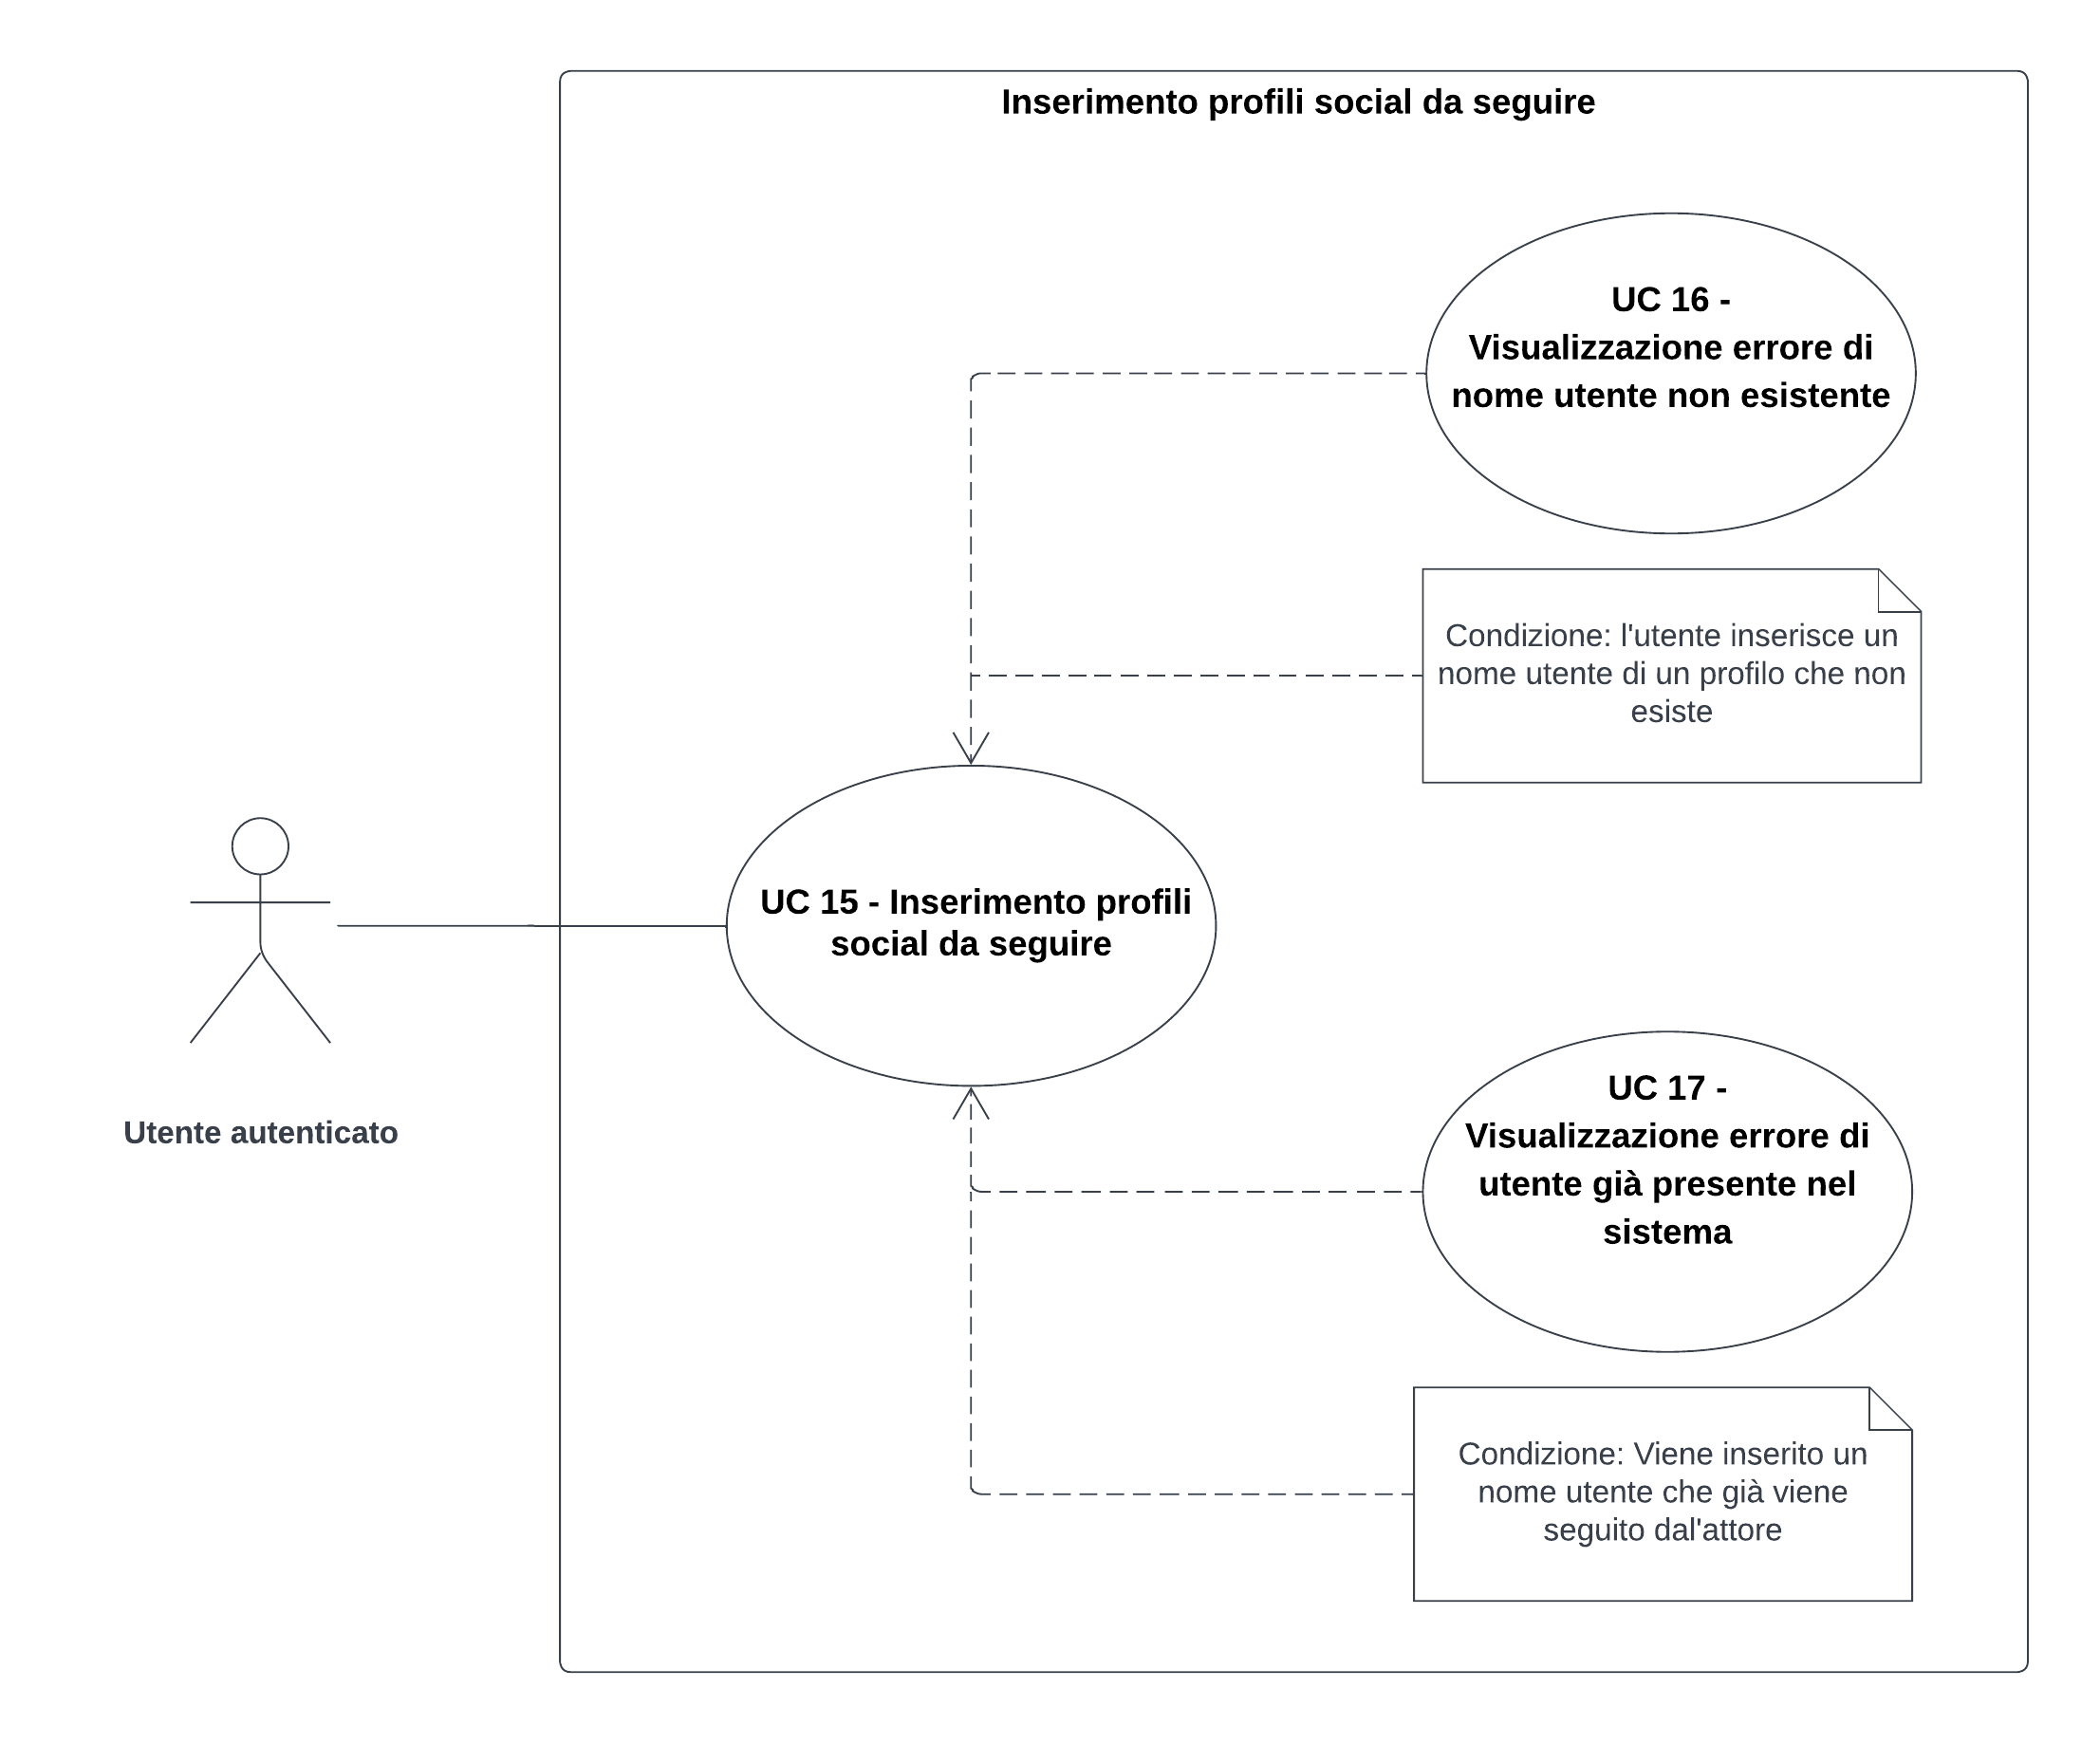
\includegraphics[width=15cm]{sezioni/Images/UC15.png}
    \centering
    \caption{Inserimento profili social da seguire}
\end{figure}

\begin{itemize}
    \item \textbf{Attore}: l'utente è autenticato.
    \item \textbf{Descrizione}: l'utente deve poter aggiungere dei profili social da seguire e da cui sarà generata la guida.
    \item \textbf{Scenario}:
    \begin{enumerate}
        \item l'utente naviga nella sezione dei profili seguiti;
        \item l'utente clicca il pulsante di aggiunta profilo;
        \item l'utente inserisce l'username da aggiungere;
        \item l'utente conferma e salva.
    \end{enumerate}
    \item \textbf{Estensioni}:
    \begin{itemize}
    	\item il profilo inserito non esiste \textbf{(UC17)};
    	\item il profilo inserito è già stato aggiunto \textbf{(UC18)}.
    \end{itemize} 
    \item \textbf{Precondizioni}: l'utente vuole seguire un nuovo utente.
    \item \textbf{Postcondizioni}: l'utente ha inserito un nuovo utente da seguire.
\end{itemize}

\subsection{UC17 - Visualizzazione errore di nome utente non esistente}
\begin{itemize}
    \item \textbf{Attore}: l'utente è autenticato.
    \item \textbf{Descrizione}: durante l'attività di aggiunta di un profilo l'utente deve ricevere un messaggio d'errore se il nome utente ricercato non è presente nel sistema.
    \item \textbf{Scenario}: l'utente legge un messaggio d'errore. 
    \item \textbf{Precondizioni}: l'utente inserisce un nome utente inesistente nella procedura di inserimento dei profili social da seguire.
    \item \textbf{Postcondizioni}: l'utente ha ricevuto un messaggio d'errore.
\end{itemize}

\subsection{UC18 - Visualizzazione errore di utente già presente nel sistema}
\begin{itemize}
    \item \textbf{Attore}: l'utente è autenticato.
    \item \textbf{Descrizione}: durante l'attività di aggiunta di un profilo l'utente deve ricevere un messaggio d'errore se il nome utente ricercato è già stato inserito nei profili seguiti dall'utente.
    \item \textbf{Scenario}: l'utente legge un messaggio d'errore. 
    \item \textbf{Precondizioni}: l'utente inserisce un nome utente nella procedura di inserimento dei profili social da seguire che è già presente tra quelli seguiti.
    \item \textbf{Postcondizioni}: l'utente ha ricevuto un messaggio d'errore.
\end{itemize}

\subsection{UC19 - Rimozione profili social seguito}

\begin{figure}[!h]
    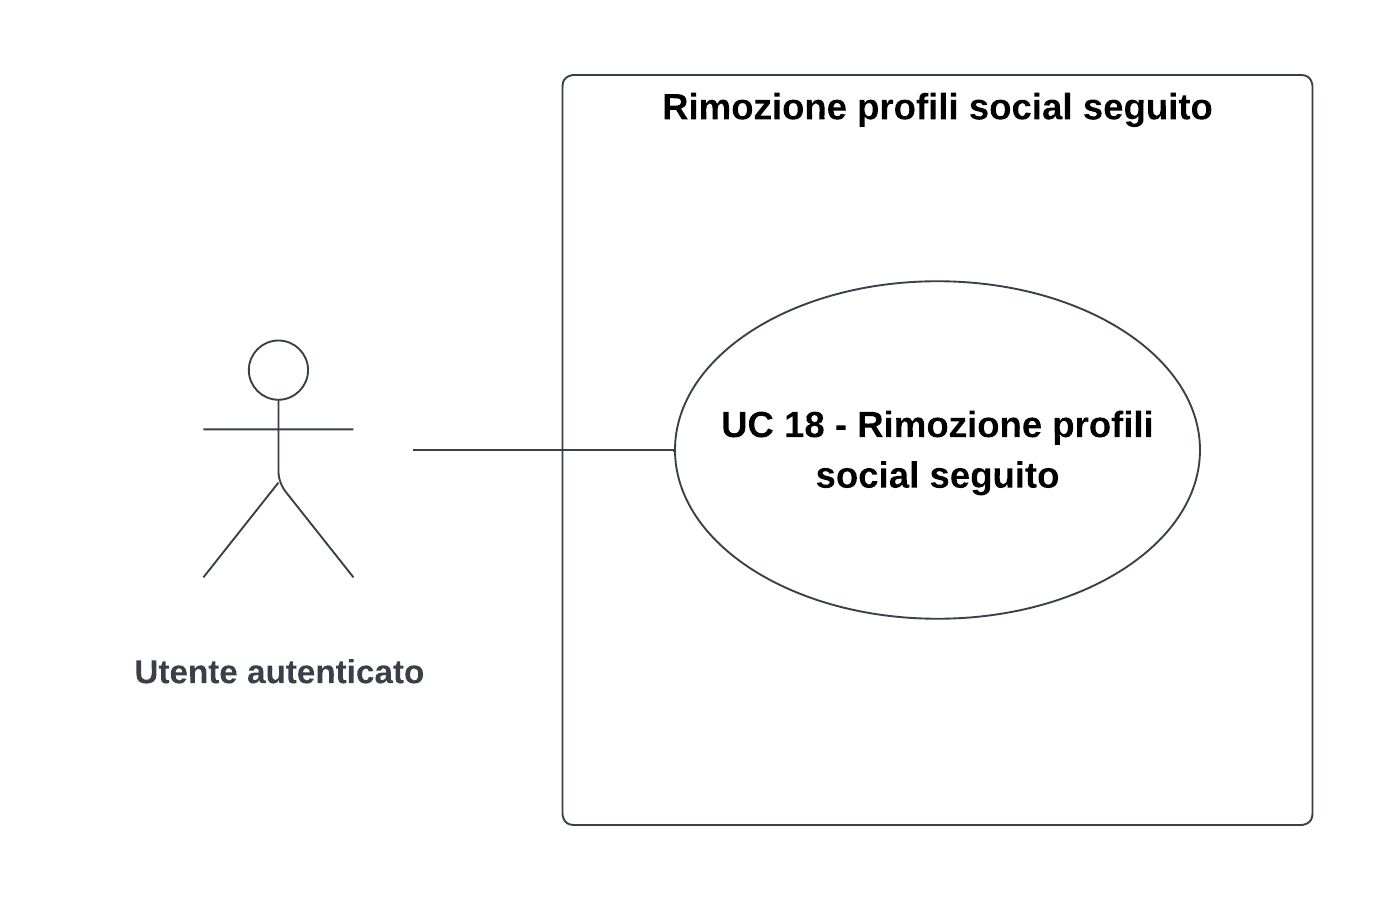
\includegraphics[width=10cm]{sezioni/Images/UC18.png}
    \centering
    \caption{Rimozione profili social seguito}
\end{figure}

\begin{itemize}
    \item \textbf{Attore}: l'utente è autenticato.
    \item \textbf{Descrizione}: l'utente deve poter rimuovere un profilo dalla lista di quelli seguiti.
    \item \textbf{Scenario}:
    \begin{enumerate}
        \item l'utente naviga nella sezione dei profili seguiti;
        \item l'utente seleziona il profilo che vuole rimuovere;
        \item l'utente clicca il pulsante di rimozione.
    \end{enumerate}

    \item \textbf{Precondizioni}: l'utente vuole rimuovere un profilo social dalla lista dei seguiti.
    \item \textbf{Postcondizioni}: l'utente ha rimosso il profilo social dalla lista dei seguiti.
\end{itemize}

\subsection{UC20 - Esplorazione profili social più seguiti}

\begin{figure}[!h]
    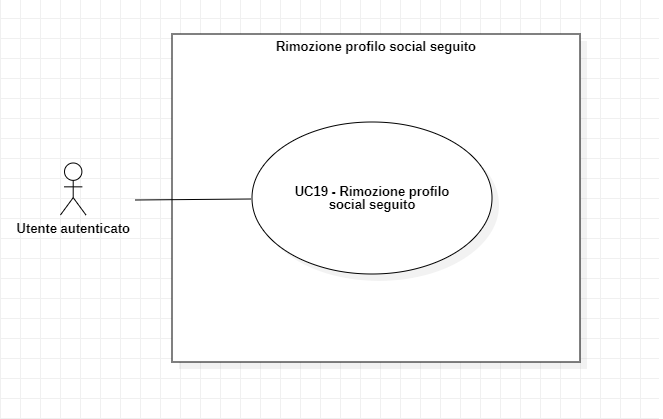
\includegraphics[width=10cm]{sezioni/Images/UC19.png}
    \centering
    \caption{Esplorazione profili social più seguiti}
\end{figure}

\begin{itemize}
    \item \textbf{Attore}: l'utente è autenticato.
    \item \textbf{Descrizione}: l'utente può esplorare i profili social più seguiti dagli altri utenti di questa piattaforma.
    \item \textbf{Scenario}:
    \begin{enumerate}
        \item l'utente si trova nella home;
        \item l'utente preme il pulsante per entrare nella pagina di esplorazione;
        \item l'utente vede la lista dei profili social più seguiti.
    \end{enumerate}
    \item \textbf{Precondizioni}: l'utente vuole visualizzare la lista dei profili social più seguiti.
    \item \textbf{Postcondizioni}: viene visualizzata all'utente la lista dei profili social più seguiti.
\end{itemize}

\subsection{UC21 - Impostazione vista predefinita guida}
\begin{figure}[!h]
    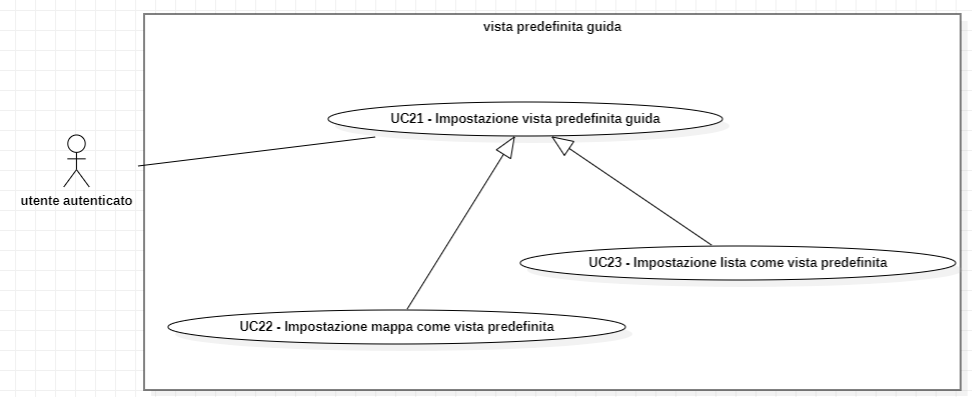
\includegraphics[width=15cm]{sezioni/Images/UC20_s.png}
    \centering
    \caption{Impostazione vista predefinita guida}
\end{figure}

\begin{itemize}
    \item \textbf{Attore}: l'utente è autenticato.
    \item \textbf{Descrizione}: l'utente deve poter scegliere la vista predefinita per visualizzare la guida.
    \item \textbf{Scenario}:
    \begin{enumerate}
        \item l'utente naviga nella sezione impostazioni;
        \item l'utente sceglie la voce “Vista predefinita”;
        \item l'utente sceglie tra la visulizzazione della mappa \textbf{(UC 22)} oppure della lista \textbf{(UC 23)}.
    \end{enumerate}

    \item \textbf{Precondizioni}: l'utente vuole poter sceglie la vista predefinita.
    \item \textbf{Postcondizioni}: la scelta della lista predefinita è stata salvata.
\end{itemize}

\subsection{UC22 - Impostazione mappa come vista predefinita}
\begin{itemize}
    \item \textbf{Attore}: l'utente è autenticato.
    \item \textbf{Descrizione}: l'utente sceglie la mappa come vista predefinita.
    \item \textbf{Scenario}: l'utente sceglie mappa come vista predefinita.
    \item \textbf{Precondizioni}: l'utente vuole scegliere mappa come vista predefinita.
    \item \textbf{Postcondizioni}: mappa viene impostata come vista predefinita.

\end{itemize}

\subsection{UC23 - Impostazione lista come vista predefinita}
\begin{itemize}
    \item \textbf{Attore}: l'utente è autenticato.
    \item \textbf{Descrizione}: l'utente sceglie la lista come vista predefinita.
    \item \textbf{Scenario}: l'utente sceglie lista come vista predefinita.
    \item \textbf{Precondizioni}: l'utente vuole scegliere lista come vista predefinita.
    \item \textbf{Postcondizioni}: lista viene impostata come vista predefinita.
\end{itemize}







	\newpage
	\section{Requisiti}
	In questa sezione sono classificati ed assegnati i requisiti seguendo la nomenclatura specificata nelle \NdP\G{}.

\subsection{Requisiti Funzionali}

{
      \setlength{\freewidth}{\dimexpr\textwidth-10\tabcolsep}
      \renewcommand{\arraystretch}{1.5}
      \centering
      \setlength{\aboverulesep}{0pt}
      \setlength{\belowrulesep}{0pt}
      \rowcolors{2}{Arancione!10}{white}
      \begin{longtable}{C{.15\freewidth} C{.2\freewidth} C{.528\freewidth} C{.15\freewidth}}
         \toprule
      \rowcolor{Arancione}
      \textcolor{white}{\textbf{Codice}}&
      \textcolor{white}{\textbf{Classificazione}}&
      \textcolor{white}{\textbf{Descrizione}}&
      \textcolor{white}{\textbf{Fonti}}\\	
      \toprule
      \endhead
      
      RF1 & Obbligatorio & L'utente deve poter registrarsi inserendo i suoi dati personali (email, nome utente e password) & UC1 \\
      RF2 & Obbligatorio & L'utente deve poter effettuare il login inserendo i dati personali richiesti (nome utente e password) & UC5 \\
      RF3 & Obbligatorio & L'utente deve poter effettuare il logout e uscire dalla sessione & UC9 \\
      RF4 & Obbligatorio & All'utente viene mostrato un messaggio d'errore se la mail inserita durante la fase di registrazione è già presente nel sistema  & UC1.1 \\
      RF5 & Obbligatorio & All'utente viene mostrato un messaggio d'errore se il nome utente inserito durante la fase di registrazione è già presente nel sistema & UC1.2 \\
      RF6 & Obbligatorio & All'utente viene mostrato un messaggio d'errore se la password inserita durante la fase di registrazione non presenta le specifiche richieste & UC1.3 \\
      RF7 & Obbligatorio & All'utente viene mostrato un messaggio d'errore se il nome utente inserito durante la fase di autenticazione è errato & UC5, UC5.1 \\
      RF8 & Obbligatorio & All'utente viene mostrato un messaggio d'errore se la email inserita durante la fase di autenticazione è errata & UC6\\
      RF9 & Obbligatorio & All'utente viene mostrato un messaggio d'errore se la password inserita durante la fase di autenticazione è errata & UC5, UC5.2 \\
      RF10 & Obbligatorio & L'utente deve poter modificare la propria password inserendo la vecchia password e confermando la nuova & UC10 \\
      RF11 & Obbligatorio & All'utente compare un messaggio d'errore se durante il cambio password, la password attuale inserita non è corretta & UC11 \\
      RF12 & Obbligatorio & All'utente compare un messaggio d'errore se durante il cambio password, la nuova password inserita non rispetta le specifiche & UC12 \\
      RF13 & Obbligatorio & All'utente compare un messaggio d'errore se durante il cambio password, la ripetizione della nuova password inserita non è uguale alla password del campo precedente & UC13 \\
      RF14 & Obbligatorio & L'utente deve poter autenticarsi automaticamente, senza inserire le credenziali & UC8\\
      RF15 & Obbligatorio & L'utente deve poter visualizzare la guida in formato mappa o formato lista & UC14, UC14.1, UC14.2, UC14.3, UC14.4 \\
      RF16 & Obbligatorio & L'utente deve poter visualizzare la mappa globale se non ha nessun profilo social seguito & UC14, UC14.1 \\
      RF17 & Obbligatorio & L'utente deve poter visualizzare la lista personalizzata se segue dei profili social & UC14, UC14.4 \\
      RF18 & Obbligatorio & L'utente deve poter visualizzare la mappa personalizzata se segue dei profili social & UC14, UC14.3 \\
      RF19 & Obbligatorio & L'utente deve poter aggiungere dei profili social da seguire, dai quali verrà generata la guida & UC15 \\
      RF20 & Obbligatorio & L'utente deve poter visualizzare un messaggio di errore nel caso in cui il nome del profilo utente inserito non esista nel sistema & UC16 \\
      RF21 & Obbligatorio & L'utente deve poter visualizzare un messaggio di errore nel caso in cui il nome del profilo utente ricercato si trova già nei profili seguiti & UC17 \\
      RF22 & Obbligatorio & L'utente deve poter rimuovere un profilo dalla lista di quelli che segue & UC18 \\
      RF23 & Obbligatorio & L'utente può esplorare gli utenti più seguiti dagli altri utenti di questa piattaforma & UC19 \\
      RF24 & Obbligatorio & L'utente deve poter scegliere la vista predefinita per visualizzare la guida & UC20 \\
      RF25 & Obbligatorio & L'utente deve poter scegliere di mettere la mappa come vista predefinita & UC20, UC20.1 \\
      RF26 & Obbligatorio & L'utente deve poter scegliere di mettere la mappa come vista predefinita & UC20, UC20.2 \\	   
      \bottomrule
      \rowcolor{white} 
      \caption{Tabella dei requisiti funzionali}
      \end{longtable}
}
\subsection{Requisiti di Vincolo}
{
      \setlength{\freewidth}{\dimexpr\textwidth-10\tabcolsep}
      \renewcommand{\arraystretch}{1.5}
      \centering
      \setlength{\aboverulesep}{0pt}
      \setlength{\belowrulesep}{0pt}
      \rowcolors{2}{Arancione!10}{white}
      \begin{longtable}{C{.15\freewidth} C{.2\freewidth} C{.528\freewidth} C{.15\freewidth}}
         \toprule
      \rowcolor{Arancione}
      \textcolor{white}{\textbf{Codice}}&
      \textcolor{white}{\textbf{Classificazione}}&
      \textcolor{white}{\textbf{Descrizione}}&
      \textcolor{white}{\textbf{Fonti}}\\	
      \toprule
      \endhead
      
      RV1 & Obbligatorio & La piattaforma deve fornire la possibilità di monitorare le recensioni partendo da un luogo indicato & Capitolato \\
      RV2 & Obbligatorio & La piattaforma deve permettere di indicare profili social da seguire per creare la guida & Capitolato \\
      RV3 & Obbligatorio & I profili social da seguire devono provenire dalle piattaforme Instagram\G{} e TikTok\G{} & Capitolato \\
      RV4 & Obbligatorio & Il backend\G{} deve essere implementato secondo un'architettura serverless\G{} & Capitolato \\
      RV5 & Obbligatorio & Il backend\G{} deve utilizzare le funzionalità di machine learning fornite dai servizi AWS\G{} & Capitolato \\
      RV6 & Obbligatorio & La piattaforma deve essere fruibile da web browser. In particolare dovrà essere garantita la compatibilità con le versioni più recenti dei browser \textit{Chrome} e \textit{Firefox}. & Capitolato \\
      RV7 & Obbligatorio & Il backend\G{} deve utilizzare le informazioni testuali di post derivati da profili social per trarre informazioni su un luogo fisico & Capitolato \\
      RV8 & Molto Desiderabile & Il backend\G{} dovrebbe utilizzare le informazioni grafiche e visuali di post derivati da profili social per trarre informazioni su un luogo fisico & Capitolato \\
      RV9 & Obbligatorio & Deve essere costruito un crawler/scraper\G{} in grado di accedere o scaricare dati dei post da profili social & Capitolato \\
      RV10 & Obbligatorio & Il crawler\G{} deve eludere i servizi anti-bot dei vari social & Capitolato \\
      \bottomrule
      \rowcolor{white} 
      \caption{Tabella dei requisiti di vincolo}
      \end{longtable}
}
\subsection{Requisiti di Qualità}
{
      \setlength{\freewidth}{\dimexpr\textwidth-10\tabcolsep}
      \renewcommand{\arraystretch}{1.5}
      \centering
      \setlength{\aboverulesep}{0pt}
      \setlength{\belowrulesep}{0pt}
      \rowcolors{2}{Arancione!10}{white}
      \begin{longtable}{C{.15\freewidth} C{.2\freewidth} C{.528\freewidth} C{.15\freewidth}}
         \toprule
      \rowcolor{Arancione}
      \textcolor{white}{\textbf{Codice}}&
      \textcolor{white}{\textbf{Classificazione}}&
      \textcolor{white}{\textbf{Descrizione}}&
      \textcolor{white}{\textbf{Fonti}}\\	
      \toprule
      \endhead
      
      RQ1 & Obbligatorio & Il sistema dovrà essere sviluppato secondo le norme descritte nel documento Norme di Progetto\G{} & Decisione Interna \\
      RQ2 & Obbligatorio & Manuale utente in lingua italiana & Decisione Interna \\
      RQ3 & Obbligatorio & Diagrammi UML\G{} relativi agli Use Cases\G{} di progetto & Capitolato \\
      RQ4 & Obbligatorio & Schema Design\G{} relativo alla base di dati & Capitolato \\
      RQ5 & Obbligatorio & Documentazione dettagliata di tutte le API\G{} & Capitolato \\
      RQ6 & Obbligatorio & Piano Unit Tests\G{} & Capitolato \\
      RQ7 & Obbligatorio & Sintesi sui limiti dei social utilizzati & Capitolato \\
      RQ8 & Obbligatorio & Limiti dei servizi e degli algoritmi usati per estrarre le valutazioni sui luoghi di interesse & Capitolato \\	   
      RQ9 & Obbligatorio & Bug Reporting & Capitolato \\
      RQ10 & Obbligatorio & Codice sorgente fornito tramite sistemi di versionamento & Capitolato \\
      \bottomrule
      \rowcolor{white} 
      \caption{Tabella dei requisiti di qualità}
      \end{longtable}
}

\newpage
\subsection{Requisiti Prestazionali}
{
      \setlength{\freewidth}{\dimexpr\textwidth-10\tabcolsep}
      \renewcommand{\arraystretch}{1.5}
      \centering
      \setlength{\aboverulesep}{0pt}
      \setlength{\belowrulesep}{0pt}
      \rowcolors{2}{Arancione!10}{white}
      \begin{longtable}{C{.15\freewidth} C{.2\freewidth} C{.528\freewidth} C{.15\freewidth}}
         \toprule
      \rowcolor{Arancione}
      \textcolor{white}{\textbf{Codice}}&
      \textcolor{white}{\textbf{Classificazione}}&
      \textcolor{white}{\textbf{Descrizione}}&
      \textcolor{white}{\textbf{Fonti}}\\	
      \toprule
      \endhead
      
      RP1 & Desiderabile & Scegliere i servizi di AWS\G{} che richiedono scambio dati nelle stesse zone geografiche & ve\_20220516 \\
      RP2 & Desiderabile & Il crawler\G/scraper\G{} dovrebbe essere efficiente e sfruttare al meglio vari servizi, come l'architettura serverless\G{} e lo spazio di archiviazione Amazon S3\G{} & Capitolato \\	   
      \bottomrule
      \rowcolor{white} 
      \caption{Tabella dei requisiti prestazionali}
      \end{longtable}
}
\subsection{Tracciamento}
\subsubsection{Fonte - Requisiti}
{
      \setlength{\freewidth}{\dimexpr\textwidth-0\tabcolsep}
      \renewcommand{\arraystretch}{1.5}
      \centering
      \setlength{\aboverulesep}{0pt}
      \setlength{\belowrulesep}{0pt}
      \rowcolors{2}{Arancione!10}{white}
      \begin{longtable}{C{.47\freewidth} C{.47\freewidth}}
         \toprule
      \rowcolor{Arancione}
      \textcolor{white}{\textbf{Fonte}}&
      \textcolor{white}{\textbf{Requisiti}}\\
      \toprule
      \endhead
      
      Capitolato & RV1, RV2, RV3, RV4, RV5, RV6, RV7, RV8, RV9, RV10,
                   RQ3, RQ4, RQ5, RQ6, RQ7, RQ8, RQ9, RQ10,
                   RP2\\
      UC1 & RF1\\
      UC1.1 & RF4\\
      UC1.2 & RF5\\
      UC1.3 & RF6\\
      UC2 & Verbale interno 20/05/2022\\
      UC3 & Verbale interno 20/05/2022\\
      UC4 & Verbale interno 20/05/2022\\
      UC5 & RF2, RF7, RF9\\
      UC5.1 & RF7\\
      UC5.2 & RF9\\
      UC5.3 & Discussione interna\\
      UC6 & RF8\\
      UC7 & RF14\\
      UC8 & RF14\\
      UC9 & RF3\\
      UC10 & RF10\\
      %UC10.1 & BOH\\
      %UC10.2 & BOH\\
      %UC10.3 & BOH\\
      %UC10.4 & BOH\\
      UC11 & RF11\\
      UC12 & RF12\\
      UC13 & RF13\\
      UC14 & RF15, RF16, RF17, RF18\\
      UC14.1 & RF15, RF16\\
      UC14.2 & RF15, RF16\\
      UC14.3 & RF15, RF18\\
      UC14.4 & RF15, RF17\\
      UC15 & RF19\\
      UC16 & RF20\\
      UC17 & RF21\\
      UC18 & RF22\\
      UC19 & RF23\\
      UC20 & RF24, RF25, RF26\\
      UC20.1 & RF25\\
      UC20.2 & RF26\\		
      \bottomrule
      \rowcolor{white} 
      \caption{Tabella fonte - requisiti}
      \end{longtable}
}
\newpage
\subsubsection{Requisito - Fonte}
{
      \setlength{\freewidth}{\dimexpr\textwidth-0\tabcolsep}
      \renewcommand{\arraystretch}{1.5}
      \centering
      \setlength{\aboverulesep}{0pt}
      \setlength{\belowrulesep}{0pt}
      \rowcolors{2}{Arancione!10}{white}
      \begin{longtable}{C{.47\freewidth} C{.47\freewidth}}
         \toprule
      \rowcolor{Arancione}
      \textcolor{white}{\textbf{Requisito}}&
      \textcolor{white}{\textbf{Fonti}}\\
      \toprule
      \endhead
      
      RF1 & UC1\\
      RF2 & UC5\\
      RF3 & UC9\\
      RF4 & UC1.1\\
      RF5 & UC1.2\\
      RF6 & UC1.3\\
      RF7 & UC5, UC5.1\\
      RF8 & UC6\\
      RF9 & UC5, UC5.2\\
      RF10 & UC10\\
      RF11 & UC11\\
      RF12 & UC12\\
      RF13 & UC13\\
      RF14 & UC7\\
      RF15 & UC14, UC14.1, UC14.2, UC14.3, UC14.4\\
      RF16 & UC14, UC14.1, UC14.2\\
      RF17 & UC14, UC14.4\\
      RF18 & UC14, UC14.3\\
      RF19 & UC15\\
      RF20 & UC16\\
      RF21 & UC17\\
      RF22 & UC18\\
      RF23 & UC19\\
      RF24 & UC20\\
      RF25 & UC20, UC20.1\\
      RF26 & UC20, UC20.2\\

      RV1 & Capitolato\\
      RV2 & Capitolato\\
      RV3 & Capitolato\\
      RV4 & Capitolato\\
      RV5 & Capitolato\\
      RV6 & Capitolato\\
      RV7 & Capitolato\\
      RV8 & Capitolato\\
      RV9 & Capitolato\\
      RV10 & Capitolato\\

      %RQ1\\
      %RQ2\\
      RQ3 & Capitolato\\
      RQ4 & Capitolato\\
      RQ5 & Capitolato\\
      RQ6 & Capitolato\\
      RQ7 & Capitolato\\
      RQ8 & Capitolato\\
      RQ9 & Capitolato\\
      RQ10 & Capitolato\\

      %RP1\\
      RP2 & Capitolato\\
      \bottomrule
      \rowcolor{white} 
      \caption{Tabella requisito - fonte}
      \end{longtable}
}


\end{document}
